% Options for packages loaded elsewhere
\PassOptionsToPackage{unicode}{hyperref}
\PassOptionsToPackage{hyphens}{url}
%
\documentclass[
  english,
  man,floatsintext]{apa7}
\usepackage{lmodern}
\usepackage{amsmath}
\usepackage{ifxetex,ifluatex}
\ifnum 0\ifxetex 1\fi\ifluatex 1\fi=0 % if pdftex
  \usepackage[T1]{fontenc}
  \usepackage[utf8]{inputenc}
  \usepackage{textcomp} % provide euro and other symbols
  \usepackage{amssymb}
\else % if luatex or xetex
  \usepackage{unicode-math}
  \defaultfontfeatures{Scale=MatchLowercase}
  \defaultfontfeatures[\rmfamily]{Ligatures=TeX,Scale=1}
\fi
% Use upquote if available, for straight quotes in verbatim environments
\IfFileExists{upquote.sty}{\usepackage{upquote}}{}
\IfFileExists{microtype.sty}{% use microtype if available
  \usepackage[]{microtype}
  \UseMicrotypeSet[protrusion]{basicmath} % disable protrusion for tt fonts
}{}
\makeatletter
\@ifundefined{KOMAClassName}{% if non-KOMA class
  \IfFileExists{parskip.sty}{%
    \usepackage{parskip}
  }{% else
    \setlength{\parindent}{0pt}
    \setlength{\parskip}{6pt plus 2pt minus 1pt}}
}{% if KOMA class
  \KOMAoptions{parskip=half}}
\makeatother
\usepackage{xcolor}
\IfFileExists{xurl.sty}{\usepackage{xurl}}{} % add URL line breaks if available
\IfFileExists{bookmark.sty}{\usepackage{bookmark}}{\usepackage{hyperref}}
\hypersetup{
  pdftitle={Ideas cascading into keystrokes -- modelling writing hesitations as finite mixture process},
  pdfauthor={Jens Roeser1, Mark Torrance1, Rianne Conijn2, \& Evgeny Chukharev3},
  pdflang={en-EN},
  pdfkeywords={Keystroke modelling; finite mixture models; Bayesian models; text composition},
  hidelinks,
  pdfcreator={LaTeX via pandoc}}
\urlstyle{same} % disable monospaced font for URLs
\usepackage{graphicx}
\makeatletter
\def\maxwidth{\ifdim\Gin@nat@width>\linewidth\linewidth\else\Gin@nat@width\fi}
\def\maxheight{\ifdim\Gin@nat@height>\textheight\textheight\else\Gin@nat@height\fi}
\makeatother
% Scale images if necessary, so that they will not overflow the page
% margins by default, and it is still possible to overwrite the defaults
% using explicit options in \includegraphics[width, height, ...]{}
\setkeys{Gin}{width=\maxwidth,height=\maxheight,keepaspectratio}
% Set default figure placement to htbp
\makeatletter
\def\fps@figure{htbp}
\makeatother
\setlength{\emergencystretch}{3em} % prevent overfull lines
\providecommand{\tightlist}{%
  \setlength{\itemsep}{0pt}\setlength{\parskip}{0pt}}
\setcounter{secnumdepth}{-\maxdimen} % remove section numbering
% Make \paragraph and \subparagraph free-standing
\ifx\paragraph\undefined\else
  \let\oldparagraph\paragraph
  \renewcommand{\paragraph}[1]{\oldparagraph{#1}\mbox{}}
\fi
\ifx\subparagraph\undefined\else
  \let\oldsubparagraph\subparagraph
  \renewcommand{\subparagraph}[1]{\oldsubparagraph{#1}\mbox{}}
\fi
% Manuscript styling
\usepackage{upgreek}
\captionsetup{font=singlespacing,justification=justified}

% Table formatting
\usepackage{longtable}
\usepackage{lscape}
% \usepackage[counterclockwise]{rotating}   % Landscape page setup for large tables
\usepackage{multirow}		% Table styling
\usepackage{tabularx}		% Control Column width
\usepackage[flushleft]{threeparttable}	% Allows for three part tables with a specified notes section
\usepackage{threeparttablex}            % Lets threeparttable work with longtable

% Create new environments so endfloat can handle them
% \newenvironment{ltable}
%   {\begin{landscape}\begin{center}\begin{threeparttable}}
%   {\end{threeparttable}\end{center}\end{landscape}}
\newenvironment{lltable}{\begin{landscape}\begin{center}\begin{ThreePartTable}}{\end{ThreePartTable}\end{center}\end{landscape}}

% Enables adjusting longtable caption width to table width
% Solution found at http://golatex.de/longtable-mit-caption-so-breit-wie-die-tabelle-t15767.html
\makeatletter
\newcommand\LastLTentrywidth{1em}
\newlength\longtablewidth
\setlength{\longtablewidth}{1in}
\newcommand{\getlongtablewidth}{\begingroup \ifcsname LT@\roman{LT@tables}\endcsname \global\longtablewidth=0pt \renewcommand{\LT@entry}[2]{\global\advance\longtablewidth by ##2\relax\gdef\LastLTentrywidth{##2}}\@nameuse{LT@\roman{LT@tables}} \fi \endgroup}

% \setlength{\parindent}{0.5in}
% \setlength{\parskip}{0pt plus 0pt minus 0pt}

% Overwrite redefinition of paragraph and subparagraph by the default LaTeX template
% See https://github.com/crsh/papaja/issues/292
\makeatletter
\renewcommand{\paragraph}{\@startsection{paragraph}{4}{\parindent}%
  {0\baselineskip \@plus 0.2ex \@minus 0.2ex}%
  {-1em}%
  {\normalfont\normalsize\bfseries\itshape\typesectitle}}

\renewcommand{\subparagraph}[1]{\@startsection{subparagraph}{5}{1em}%
  {0\baselineskip \@plus 0.2ex \@minus 0.2ex}%
  {-\z@\relax}%
  {\normalfont\normalsize\itshape\hspace{\parindent}{#1}\textit{\addperi}}{\relax}}
\makeatother

% \usepackage{etoolbox}
\makeatletter
\patchcmd{\HyOrg@maketitle}
  {\section{\normalfont\normalsize\abstractname}}
  {\section*{\normalfont\normalsize\abstractname}}
  {}{\typeout{Failed to patch abstract.}}
\patchcmd{\HyOrg@maketitle}
  {\section{\protect\normalfont{\@title}}}
  {\section*{\protect\normalfont{\@title}}}
  {}{\typeout{Failed to patch title.}}
\makeatother
\shorttitle{Modelling writing hesitations}
\keywords{Keystroke modelling; finite mixture models; Bayesian models; text composition}
\usepackage{csquotes}
\usepackage{booktabs}
\usepackage{longtable}
\usepackage{graphicx}
\usepackage{array}
\usepackage{multirow}
\usepackage{float}
\usepackage{colortbl}
\usepackage{threeparttable}
\usepackage[normalem]{ulem}
\usepackage[utf8]{inputenc}
\usepackage{icomma}
\usepackage{pdflscape}
\newcommand{\blandscape}{\begin{landscape}}
\newcommand{\elandscape}{\end{landscape}}
\DeclareCaptionFormat{cont}{#1 (cont.)#2#3\par}
\ifxetex
  % Load polyglossia as late as possible: uses bidi with RTL langages (e.g. Hebrew, Arabic)
  \usepackage{polyglossia}
  \setmainlanguage[]{english}
\else
  \usepackage[shorthands=off,main=english]{babel}
\fi
\ifluatex
  \usepackage{selnolig}  % disable illegal ligatures
\fi
\newlength{\cslhangindent}
\setlength{\cslhangindent}{1.5em}
\newlength{\csllabelwidth}
\setlength{\csllabelwidth}{3em}
\newenvironment{CSLReferences}[2] % #1 hanging-ident, #2 entry spacing
 {% don't indent paragraphs
  \setlength{\parindent}{0pt}
  % turn on hanging indent if param 1 is 1
  \ifodd #1 \everypar{\setlength{\hangindent}{\cslhangindent}}\ignorespaces\fi
  % set entry spacing
  \ifnum #2 > 0
  \setlength{\parskip}{#2\baselineskip}
  \fi
 }%
 {}
\usepackage{calc}
\newcommand{\CSLBlock}[1]{#1\hfill\break}
\newcommand{\CSLLeftMargin}[1]{\parbox[t]{\csllabelwidth}{#1}}
\newcommand{\CSLRightInline}[1]{\parbox[t]{\linewidth - \csllabelwidth}{#1}\break}
\newcommand{\CSLIndent}[1]{\hspace{\cslhangindent}#1}

\title{Ideas cascading into keystrokes -- modelling writing hesitations as finite mixture process}
\author{Jens Roeser\textsuperscript{1}, Mark Torrance\textsuperscript{1}, Rianne Conijn\textsuperscript{2}, \& Evgeny Chukharev\textsuperscript{3}}
\date{}


\authornote{

Correspondence concerning this article should be addressed to Jens Roeser, 50 Shakespeare St, Nottingham NG1 4FQ. E-mail: \href{mailto:jens.roeser@ntu.ac.uk}{\nolinkurl{jens.roeser@ntu.ac.uk}}

}

\affiliation{\vspace{0.5cm}\textsuperscript{1} Department of Psychology, Nottingham Trent University, United Kingdom\\\textsuperscript{2} Artificial Intelligence Systems Institute, Eindhoven University of Technology, The Netherlands\\\textsuperscript{3} Department of English, Iowa State University, Iowa}

\abstract{
Classical serial models view the process of producing a text as a descrete chain of pauses and writing bursts. In contrast, parallel cascading models of writing assume that planning is not complete at production onset and operates in parallel to writing execution. We implemented these two view in Bayesian statistical models and applied our models to key-stroke logs of 6 data sets from free text production. We reanalysed keystroke intervals at before-sentence transitions, before word transitions and within word transitions. Model comparisons demonstrated strong evidence in favour of the statistical implementation of the cascading view of the serial models across all data sets. Further we found that although pause durations are consistently longer for larger linguistic edges, the pause frequencies are not, but largely identical for before sentence and before word transition locations. Our results cannot be explained by the serial but are in line with the cascading view of writing.
}



\begin{document}
\maketitle

Translating ideas into language involves a cascade of processes starting with a communicative intention, over the generation of an message, deciding with which part of the message to start the utterance, retrieving appropriate lexical materials and ordering them in an appropriate syntactic order before retrieving orthographic and / or phonological codes that are finally submitted to the motor programs that allow us to articulate language in speech, keyboard tying, handwriting, and signing (Bock \& Ferreira, 2014; Olive, 2014; Van Galen, 1991; Wheeldon \& Konopka, 2023).

Writing is arguably more demanding than spoken language, because, among other reasons, writing requires spelling and we typically do not move our fingers or our pen as quickly as we articulate language sounds in speech. Consequently in writing more than in speech, we have to mentally buffer our linguistic plan before we can express it in language. Written communication is also less time constrained: speaking underlies fluency requirements and therefore has stronger pressure to plan information ahead of speaking (Roeser et al., 2019; Torrance \& Nottbusch, 2012). This is because in spoken production there is a pressure for fluency whereas hesitations in written output have no communicational implications for the reader (e.g. Clark \& Fox Tree, 2002). Indeed writers can pause when -- even in the middle of a word -- and for how long they want (within reason) without compromising communication. Written text production -- for example argumentative texts -- is therefore a combination for relatively fluent production bursts followed by pauses (Chenoweth \& Hayes, 2001).

The study reported in this paper presents a comparison of two theories of how cognitive planning processes are coordinated in writing using implementations in statistical models. On the basis of those statistical models applied to 6 datasets, we revisit the often reported finding that edges of larger linguistic units are associated with longer pauses (Conijn et al., 2019; Flower \& Hayes, 1981; Matsuhashi, 1981; Wengelin, 2006). For example, sentence boundaries are generally thought of as involving longer pauses, compared to word boundaries, because participants engage in higher-level planning (Baaijen et al., 2012; Medimorec et al., 2017; Medimorec \& Risko, 2017; Roeser et al., 2019). The same is generally observed for spoken utterances (E.-K. Lee et al., 2013; Meyer, 1996; Wheeldon et al., 2013) with some exceptions (Griffin, 2001). We first discuss pause patterns in text production and introduce two possible cognitive frameworks in which these can be interpreted. Pause-patterns at linguistic edges are important, as they are symptomatic for the two cognitive theories of writing we discuss in the following.

Written text production is the result of a cascade of processes that starts with an communicative idea on the top forming a semantic representation, which is then fed into a grammatical encoder that is responsible for the retrieval of lexical names and, depending on theoretical viewpoint (Bock \& Ferreira, 2014; Wheeldon \& Konopka, 2023), the generation of syntactic representations, and finally flow from orthographic retrieval into motor plans for executing finger movements (Olive, 2014; Van Galen, 1991). The intervals between adjacent keystrokes during typing vary as a function of various factors. Explaining the factors that influence the duration of inter-keystroke intervals (IKI) requires a theory of how the various processes that transform intent into keypresses are structured. Processing may be serial. This means that the processing cascade operates on one unit at a time. Processing of the next unit can only start when the previous unit was fully processed from communicative intention to completion of the written output. Therefore longer IKIs represent periods when the writer is planning what to write next. The subsequent burst of fluent output is then the result this planning (Alves \& Limpo, 2015; Hayes, 2012; Kaufer et al., 1986; Matsuhashi, 1981; Schilperoord, 2002). This is particularly reflected in the model proposed by Flower and Hayes (1980) that characterises the writing process as a sequence of generating ideas, planning the text, translating the ideas into language, executing hand-writing or typing, and revising the texts (also Chenoweth \& Hayes, 2001, 2003).

This serial account is consistent with the finding that average IKI duration immediately before sentence-initial keystrokes are longer than before words and these are, in turn, longer than between mid-word key presses (Mohsen, 2021; Torrance, Rønneberg, et al., 2016; Wengelin, 2002). However this account is not consistent with what we know about writing. Consider these two observations:

First, utterances are not fully formed at production onset. Instead, syntax and lexical content and even details of the message itself are planned as the emergent result of in real-time process. This is well known for spoken production (e.g. Bock \& Ferreira, 2014). For writing, there is evidence that the time to keystroke / pen onset increases when a sentence starts with a more complex sentence-initial phrases {[}Nottbusch (2010); dam09; Roeser et al. (2019){]}. For example, in Roeser et al. (2019) participants described moving arrays of images in simple utterances such as \emph{A and the B moved above the C} that either started with a conjoined noun phrase (i.e.~\emph{A and the B moved}) or a simple noun (i.e., \emph{A moved above the B and the C}). Importantly while the overall complexity of the utterance (in terms of length, number of phrases and noun) was held constant, sentences that started with a conjoined noun phrase increased the time to typing onset. This is not what one would expect if writers plan sentences (or even phrases) in full before production onset. In fact, eye movement data reported in Torrance and Nottbusch (2012) and Roeser et al. (2019) demonstrate that writers do not plan the lexical form of the utterance beyond the first noun before production onset (similar to speech Griffin, 2001, 2003), although there was evidence that lexical pre-planning of the second noun (i.e.~\emph{the B}) was more likely for conjoined noun phrases.

Second, even though average sentence-initial IKIs tends to be longer, they still tend to be very rapid. For example, Medimorec and Risko (2017) found that, in undergraduate students writing on familiar topics 71\% of sentence-initial IKIs were less than 1 sec in duration. Also Rønneberg et al. (2022) reported that sentence-initial hesitations are rare, with over 50\% of sentences preceded by very short pauses (around 430 msecs) and a mean of 1.2 seconds for the remainder of pauses. For comparison, this is less than mean written naming response latency for single objects (Torrance et al., 2018) and short sentences when describing arrays of images (Roeser et al., 2019) in a similar population. Despite the fact that writers can in principle pause when they want to, written composition is often remarkably fluent. The finding that sentence-initial IKIs are longer before words, maps onto a theory that assumes that planning a sentence requires the writer to pause and think before pressing the sentence-initial key.

If utterances are not planned in full prior to writing onset, how is it possible that at least for reasonably competent writers producing composition often occurs remarkably fluently, with very few hesitations. The two examples above and similar findings point towards much of the mental activity associated with composition, including the relatively complex processing required to plan sentences, occurring as a result of a cascade of processes that occur partly in parallel and largely without executive control. Consistent with general trends in language processing theory (Bock \& Ferreira, 2014; Chang et al., 2006; Dell et al., 2007), several researchers have argued that the processes associated with written production run at least in part in parallel (Bonin et al., 2012; Crump \& Logan, 2010; Olive, 2014; Roux et al., 2013; Van Galen, 1991). Van Galen (1991), for example, argued for a cascade of modular processes, each responsible for a specific transformation (semantic, syntactic, and so forth), with processing occurring as soon as information from the immediately upstream process becomes available (Christiansen \& Chater, 2016). Buffers provide transient storage at each processing level to accommodate unsynchronised output rates: when lower level processes lag behind higher level processes, buffers allow our fingers to catch up with thought and language related processes. In other words, when writers move from one sentence to another without hesitation this is due to planning the next sentence, to some extent, while completing output of the previous sentence.

This cascaded account of the composition process gives a rather different understanding of inter-keystroke intervals. IKIs result from one of two data-generating processes. When upstream processes output at a rate equal to or faster than can be used for finger movement planning then IKIs are determined just by time needed for executing finger movements (i.e.~just by processing below the last buffer in the processing cascade). However if one or more upstream processes provide output more slowly then IKIs become dependent directly on upstream processing times and not on finger movement. IKIs therefore form two distributions, one associated with rapid, fluent output, and another that forms as a result of delays caused by some combination of processing at the semantic, syntactic, lexical, or orthographic levels (Roeser et al., 2021).

For example, Roeser et al. (2021) demonstrated -- using a similar approach as used in the present paper -- how this mixture of distributions that results from the same underlying data generating process can be implemented using Bayesian statistical mixture modelling. In particular they analysed a large sample of copy-task data using commonly used statistical models and compared their out-of-samples predictive performance to a mixture model approach. Not only did they find substantially stronger performance for their mixture model approach but they also demonstrated that mixture models allowed them to capture the process that generates IKIs in a copy-task context in three parameters: (1) the average speed of fluent key transitions, (2) the slowdown for hesitant key presses, and (3) the probability of hesitant as opposed to fluent transitions. As argued by the authors, copy-typing underlies a similar cascade of processes as free text composition. Instead of context generation and grammatical encoding, copy-typing involves a mixture of visual encoding of the target string and mental buffering prior to the activation of motor codes. For similar approaches see Almond et al. (2012), Baaijen et al. (2012), Chenu et al. (2014), Guo et al. (2018), Hall et al. (2022), Li (2021), and Van Waes et al. (2021).

The cascading account provides an explanation for why writers sometimes pause before onsetting a sentence (or word) but often are not. This is not because in some cases sentences are not planned, or planning was postponed until after sentence onset, but that this planning was completed in parallel with previous output.

Hesitations in writing have potential disadvantages. Writers can, as we have noted, pause at any point without this affecting the eventual communicative effect of their text. However language processing is subject to what Christiansen and Chater (2016) describe as a fundamental \enquote{now-or-never} bottleneck. Buffering is transient and as a consequence of written (and spoken) production are just-in-time systems: Production must flow down the cascade of processes from message to finger movements without significant interruptions. If there is delay -- if, for example, a writer struggles to retrieve the right word or its spelling -- there is a risk that output from upstream processes, and particularly the chain of ideas that the writer wanted to communicate, will be lost. Rønneberg et al. (2022) coined this possibility the \enquote{process-disruption hypothesis.}

In the study that is presented in this paper we test using Bayesian statistical hierarchical models of keystroke intervals -- similar to Roeser et al. (2021) -- whether the cascading view of writing generalises to contexts in which participants compose texts. On the basis of these statistical models of text composition, we appraise to what extent linguistic edges (sentence and word boundaries) are associated with different pausing behaviours as frequently suggested in the literature (Ailhaud et al., 2016; Ailhaud \& Chenu, 2017; Chukharev-Hudilainen et al., 2019; Conijn et al., 2019; Mohsen, 2021; Torrance, Rønneberg, et al., 2016; Wengelin, 2002).

Data form spontaneous text production (see Gernsbacher \& Givón, 1995) are an ideal test case for our modelling approach for the following three reasons: First, text production such as essay, argumentative, and narrative writing in response to a writing brief or topic statement is a natural environment for text production. Therefore our models have real-world relevance for educators, for example, to evaluate to what extent a student is using a desirable composition strategy (Dux Speltz et al., 2022; Dux Speltz \& Chukharev-Hudilainen, 2021; Vandermeulen et al., 2023).

Second, since the emergence of software such as InputLog (Leijten \& Van Waes, 2013) recording keystroke data during free text composition has become widely used among writing researchers and led to a rapidly expanding timecourse literature with a focus on the orchestration of subprocesses; with a recent special issue in Reading and Writing (Conijn \& Torrance, 2023). Social Science Citation Index reports 40 journal papers that describe research exploring composition processes using keystroke logging methods in 2022, compared to 26 in 2017 to 2019, and 7 in 2014 to 2016. These data are therefore important for contemporary theories of writing and freely available for modelling and machine learning (Conijn et al., 2019; Conijn, 2020).

Third, data from spontaneous text production allow us to address questions about sentence production in context that would not be possible with data from, for example, picture description experiments (Damian \& Stadthagen-Gonzalez, 2009; Nottbusch, 2010; Roeser et al., 2019) or copy tasks (Roeser et al., 2021; Van Waes et al., 2019, 2021). In text composition, content generation is not artificially constrained to individual sentence units (or less) by one or more images -- as in sentence-elicitation studies -- and linguistic form is not constraint to a sequence of words -- as in copy tasks. Instead text composition provides data from both inter and intra-sentence transitions. Also, pauses do not reflect visual encoding of the stimulus (although possibly looking back during writing which we will return to in the discussion).

The hypotheses are as follows: if the preparation of the upcoming production unit happens entirely at the corresponding linguistic edge as predicted by the serial account, and not in parallel to production, key-transition intervals can statistically be modelled as a function of the associated transition location. In other words, we expect IKIs to be proportionally longer at before-sentence locations compared to before-word location compared to within-word locations. This is because transitions before larger linguistic units are associated with processing that involves higher levels of representation. The cascading view, in contrast, assumes that although IKIs at larger linguistic edges might be longer, it is in principle possible that writers do not pause but plan in parallel to writing. In other words, statistical models of the pause-and-burst view of written production do not capture that planning can operate, to some extent, in parallel to the output of the written production. Therefore, a statistical model that captures writing as a cascade of processes must account for the possibility that hesitations occure probabilistic across the entire text although some linguistic locations such as larger linguistic edges are associated with a higher pausing probability. We hypothesize that the statistical model of the parallel cascading view provides a better out-of-sample generalization than the implementation of the serial model of writing in the context of unconstrained text composition.

\hypertarget{methods}{%
\section{Methods}\label{methods}}

We (re)analysed keystroke data of 6 experiments in which participants composed text in a series of 5 Bayesian models. The first three models map onto the serial account of writing hesitations and bridge between commonly used statistical models for the analysis of inter-keystroke intervals (IKI) as single distribution models. In particular we used a Gaussian distribution, a log-normal model, and an unequal variance model that takes into consideration that longer latencies -- those associated with larger linguistic edges -- are known to be associated with a larger variance component (Schöner, 2002; Wagenmakers \& Brown, 2007; Wing \& Kristofferson, 1973).

The remaining two models are implementations of the cascading view following the two-distributions mixture-model approach presented in Roeser et al. (2021). Importantly these two models assume that IKIs result from a mixture of two processes: (1) uninhibited activation flow into motor programmes and (2) interruptions at higher levels cause delays in the information flow. Importantly these two models assume that hesitations are not sufficiently determined by transition location -- as the serial account does -- but also transition locations are associated with different probabilities that hesitation may occur. This view was implemented as a constrained and an unconstrained model.

We reanalysed datasets from six experiments in which researchers elicited full texts in response to writing prompts. We discussed advantages with this approach in the introduction section. These datasets include samples from populations with different writing experience and languages (e.g.~young / L2 writers, students) and writing tasks (e.g.~essays, syntheses). Datasets from a variety of different writers and writing tasks were deliberately chosen to challange our modelling approach and to test to what extent resulting pausing patterns generalise across writing contexts.

\hypertarget{data-sets}{%
\subsection{Data sets}\label{data-sets}}

Six datasets with keystroke data from free text production were used for analysis. An overview can be found in Table \ref{tab:datasets}; details will be presented below.

\begin{landscape}

\begin{table}[tbp]

\begin{center}
\begin{threeparttable}

\caption{\label{tab:datasets}Datasets in brief.}

\footnotesize{

\begin{tabular}{llllrrp{2cm}p{3cm}}
\toprule
Dataset & \multicolumn{1}{c}{Source} & \multicolumn{1}{c}{Keylogger} & \multicolumn{1}{c}{Writing task} & \multicolumn{1}{c}{N (ppts)} & \multicolumn{1}{c}{Mean age} & \multicolumn{1}{c}{Language} & \multicolumn{1}{c}{Manipulation}\\
\midrule
C2L1 & Rønneberg et al. (2022) & EyeWrite & Argumentative essays & 126 & 11.80 & Norwegian & --\\
CATO & Torrance et al. (2016) & EyeWrite & Expository texts & 52 & 16.90 & Norwegian & weak decoders / control; masked / unmasked\\
GUNNEXP2 & Torrance and Ofstad (n.d) & EyeWrite &  & 45 & NA & Norwegian & masked / unmasked\\
LIFT & Vandermeulen, Steendam, et al. (2020) & InputLog & Synthesis & 658 & 16.95 & Dutch & Various topics and genres\\
PLanTra & Rossetti and Van Waes (2022b) & InputLog & Text simplification & 47 & 23.00 & English (L2) & pre / post test trained in plain language principles and control\\
SPL2 & Torrance et al. (n.d.) & CyWrite & Argumentative essays & 39 & 20.60 & English (L1) / Spanish (L2) & write in L1 / L2\\
\bottomrule
\end{tabular}

}

\end{threeparttable}
\end{center}

\end{table}
\end{landscape}

TODO: Mark, can you add information for C2L1 and CATO as needed

TODO: might need to remove kids that don't speak Norwegian at home (see github issue)? I don't think that's necessary though.

For C2L1, CATO, and GUNNEXP2, keystroke data were captured using EyeWrite (Simpson \& Torrance, 2007; Torrance, 2012).

The C2L1 dataset comprises data Norwegian 6th graders -- \emph{N} = 126, mean age 11 years 10 months -- published in Rønneberg et al. (2022). The children composed argumentative essays in Norwegian, a language with a relatively shallow orthography.

The CATO dataset is published in Torrance, Rønneberg, et al. (2016). Norwegian upper secondary students -- \emph{N} = 26, mean age = 16.9 years -- with weak decoding skills and 26 age-matched controls composed expository texts by keyboard under two conditions: normally and with letters masked to prevent them reading what they were writing.

TODO: Mark, can you add information here? I've added a provisional bib entry that needs changing or we just say \enquote{unpublished.} I could also just use Escop as reference (also for SPL2; maybe my SIG Writing talk). Was the sample Norwegian?

The GUNNEXP2 dataset published in Torrance and Ofstad (n.d.) includes keystroke data from a text composition task performed by Norwegian undergraduate students (mean age: XXX). In this dataset participants wrote texts either in a masked condition in which the produced text was replaced by 'x's or in an unmasked condition in which the students composed text as normal.

The SPL2 data set involves undergraduate university students in the US -- \emph{N} = 39, 2mean age = 20.6 years, SD = 1.51 -- composing argumentative essays in English (L1) and Spanish (L2). Students wrote within the CyWrite word-processing environment (Chukharev-Hudilainen et al., 2019). Participants wrote, with a 40 minute time limit, to two writing prompts. Order and writing prompt were counterbalanced across language.

LIFT and PLanTra data data were captured using InputLog (Leijten \& Van Waes, 2013; Van Waes et al., 2019, 2021).

The LIFT data are published in Vandermeulen, Steendam, et al. (2020) and described in Vandermeulen, De Maeyer, et al. (2020). LIFT is a representative sample of Dutch students (\emph{N} = 658, mean age = 16.95 years, 428 females and 230 males) in the three highest grades of pre-university education collected from 43 schools. The students were asked to conduct four synthesis writing tasks, two argumentative and two informative texts, about each of four topics, with order randomized per school. The students received 50 minutes for each tasks.

The PLanTra (Plain Language Training for business content) data are published in Rossetti and Van Waes (2022b) and described in Rossetti and Van Waes (2022a). The primary aim of the project was to investigate the impact of plain language instruction on business students' strategies to simplify business texts as well as on the comprehensibility of the produced texts. A total of \emph{N} = 47 graduate students (mean age = 23 years, 38 females and 9 males, 45 native Dutch speakers) of the master Business and Economics participated. The study adopted a pre-test post-test design. As pre-test, participants were asked to rewrite a given text (extract of a corporate report on sustainability), to make it more engaging and easier to read for a lay audience. Thereafter the experimental group received online instruction on how to apply plain language principles to sustainability content, while the control group received online instruction exclusively on the topic of sustainability. Participants were asked to spend at least 45 minutes on the instruction module. As post-test, participants were asked 2-3 days later to simplify another extract of a corporate report on sustainability. Both reports were written in English (second language) and similar in length (274-278 words) and readability. Participants received as much time as needed for each task.

TODO: Mark, can you add information here?

The SPL2 dataset is published in Torrance et al. (n.d.). The data come from a text composition task of undergraduate university students -- \emph{N} = 39, 28 female, mean age = 20.6 years (SD = 1.51) -- who wrote two short argumentative essays, one in English (the student's first language in all cases; L1) and one in Spanish (L2) using CyWrite (Chukharev-Hudilainen et al., 2019). Participants wrote essays in response to each of two prompts, with order and L1 / L2 counterbalanced across subjects.

\hypertarget{transition-types}{%
\subsection{Transition types}\label{transition-types}}

The transition types that were analysed in this study focus on those locations that were found, by previous research, to be psycholinguistically meaningful (Chukharev-Hudilainen et al., 2019; De Smet et al., 2018; Torrance et al., n.d.; Torrance, Rønneberg, et al., 2016) and are detailed in Table \ref{tab:keyloc}. In particular we analysed the key-transitions that resulted in the insertion of a character that started a new sentence as before-sentence transition; transitions that started a new word other than those at the beginning of a sentence were treated as before-word transition; all transitions within a word but not the key-transition between the last letter of a word and the subsequent space or punctuation mark were treated as within-word transitions. At before-sentence locations, IKIs were timed to the shift keypress for most data sets (CATO, C2L1, SPL2, GUNNEXP2) but included the transition to the following sentence-initial letters in some data sets (PLanTra, LIFT); we will return to this issue in the Results section. Transitions that occurred at the beginning of the text or the beginning of a paragraph were not treated as before-sentence transitions and were removed from the analysis.

\begin{table}[tbp]

\begin{center}
\begin{threeparttable}

\caption{\label{tab:keyloc}Transition location classification.}

\footnotesize{

\begin{tabular}{p{3cm}p{3cm}p{8cm}}
\toprule
Transition type & \multicolumn{1}{c}{Description} & \multicolumn{1}{c}{Example}\\
\midrule
Within word & Transitions between any letter & T$^{\wedge}$h$^{\wedge}$e c$^{\wedge}$a$^{\wedge}$t m$^{\wedge}$e$^{\wedge}$o$^{\wedge}$w$^{\wedge}$e$^{\wedge}$d. T$^{\wedge}$h$^{\wedge}$a$^{\wedge}$t[bsp][bsp]e$^{\wedge}$n i$^{\wedge}$t s$^{\wedge}$l$^{\wedge}$e$^{\wedge}$p$^{\wedge}$t.\\
Below word & Keypress after space followed by any letter & The $^{\wedge}$cat $^{\wedge}$meowed. That[bsp][bsp]en $^{\wedge}$it $^{\wedge}$slept.\\
Before sentence & Keypress following a space preceding any letter & The cat meowed. $^{\wedge}$That[bsp][bsp]en it slept.\\
\bottomrule
\addlinespace
\end{tabular}

}

\begin{tablenotes}[para]
\normalsize{\textit{Note.} $'^{\wedge}$' marks transition location; [bsp] represents backspace.}
\end{tablenotes}

\end{threeparttable}
\end{center}

\end{table}

\hypertarget{data-reduction}{%
\subsection{Data reduction}\label{data-reduction}}

For all datasets we only used transitions that were not followed by an editing operation. Transitions that occurred at the beginning of the text or the beginning of a paragraph were removed. We removed participants that did not complete all conditions in studies with within-participant factors (reducing the number of participants to 343 in the LIFT data set, and 41 participants in the PLanTra data set). We removed participants that produced less than 10 sentences (LIFT: 109 participants; PLanTra: 3 participants; SPL2: 1 participant).

We further removed keystroke intervals that are extremely short (\(\le\) 50 msecs) or extremely long (\(\ge\) 30 secs); the percentage of remove keystroke data can be found in Table \ref{tab:datareduction}. From the remaining data we randomly sampled 100 observations per participant, per condition, and per transition location, with the exception of the LIFT data set. This was done for computational reasons to reduce the time the Bayesian models -- decribed in the next section -- require to complete sampling. For the LIFT data set we reduced the number of participants to 100 which is substantially more than most of the other data sets in our data pool. Because the LIFT data set included the large number of writing tasks as fixed effect, we sampled 50 observations per condition, location and participant to not exceed our computational resources. The percentage of keystroke data that went into the final analysis can be found, by transition location, in Table \ref{tab:datareduction}.

\begin{table}[bp!]

\begin{center}
\begin{threeparttable}

\caption{\label{tab:datareduction}Data reduction. Mean percentage of extreme data removed and the mean percentage of randomly sampled data by transition location. Standard error is shown in parentheses.}

\begin{tabular}{lrrrrr}
\toprule
 \multicolumn{1}{c}{ } & \multicolumn{2}{c}{Extreme values in \%} & \multicolumn{3}{c}{Randomly sampled data in \%} \\
\cmidrule(r){1-1} \cmidrule(r){2-3} \cmidrule(r){4-6}
Dataset & \multicolumn{1}{c}{$\le$ 50 msecs} & \multicolumn{1}{c}{$\ge$ 30 secs} & \multicolumn{1}{c}{within word} & \multicolumn{1}{c}{before word} & \multicolumn{1}{c}{before sentence}\\
\midrule
C2L1 & 0.19 (0.1) & 0.07 (0.06) & 35.1 (2.6) & 84.5 (1.8) & 100 (0)\\
CATO & 0.65 (0.15) & 0.02 (0.02) & 14.9 (0.9) & 48.6 (2.2) & 100 (0)\\
GUNNEXP2 & 2.16 (0.17) & 0.01 (0.01) & 6.2 (0.4) & 22.5 (1.4) & 100 (0)\\
LIFT & 2.65 (0.16) & 0 (0) & 3.2 (0.2) & 13.1 (0.9) & 99.4 (0.1)\\
PLanTra & 2.49 (0.41) & 0.04 (0.03) & 9.7 (0.6) & 36.6 (1.9) & 100 (0)\\
SPL2 & 2.29 (0.2) & 0.03 (0.02) & 5.7 (0.4) & 22.6 (1.4) & 100 (0)\\
\bottomrule
\end{tabular}

\end{threeparttable}
\end{center}

\end{table}

\hypertarget{bayesian-statitical-modelling}{%
\subsection{Bayesian statitical modelling}\label{bayesian-statitical-modelling}}

We reanalysed keystroke data -- transition durations measured as the time between first and second keypress -- from six datasets in a series of five Bayesian models. An overview of all models can be found in Table \ref{tab:models}. More detailed model descriptions and motivations can be found in Appendix \ref{statistical-models}.

\begin{table}[tbp]

\begin{center}
\begin{threeparttable}

\caption{\label{tab:models}Overview of typing-process models. All models were fitted with random intercepts for participants.}

\begin{tabular}{lp{13cm}}
\toprule
Models & \multicolumn{1}{c}{Description}\\
\midrule
M1 & Standard single Gaussian model with effects of transition location by study-specific manipulations and by-participant random effect\\
M2 & Single distribution log-Gaussian model equivialent to M1\\
M3 & Equivialent to M2 but with different variance components for each transition location (unequal variance)\\
M4 & Two-distributions mixture of a log-Gaussian of fluent intervals and another of hesitant; distribution of hesitant keystroke intervals is equivialent to M3 but distribution of fluent intervals has a mean across all design cell. Mixing proportion captures the relative number of disfluent transitions\\
M5 & Equivialent to M4 but distribution of fluent transitions is allowed to vary by transition location\\
\bottomrule
\end{tabular}

\end{threeparttable}
\end{center}

\end{table}

Models M1, M2, and M3 are single distribution models -- consistent with the serial account -- include fixed effects for each combination of transition location and dataset specific manipulations and random effects for participants. In particular models M1 and M2 are consistent with standard models used in the literature and therefore serve as baseline models. For model M3 we relaxed the equal variance assumption for transition locations, thus allowing each transition location to assume a different standard deviation (see Appendix \ref{statistical-models} for rationale).

Models M4 and M5 and extensions of the single distribution models. Importantly models M4 and M5 assume that keystroke data are the result of a combination of two data generating processes -- consistent with the cascading account -- rather than one. These are called finite mixture models in the literature (Gelman et al., 2014; MacLahlan \& Peel, 2000; Roeser et al., 2021).

These models extend the assumption that processing at higher levels of activation lead to longer pauses. Instead of assuming that there is one process that shifts the distribution of IKIs of larger linguistic edges, we introduce the assumption that pauses at larger linguistic edges are more likely but not obligatory. This is achieved by modelling IKIs as coming from a weighted mixture of two distributions associated with two different states:

\begin{enumerate}
\def\labelenumi{\arabic{enumi}.}
\item
  Activation can flow into keystrokes without interruption. These fluent keystroke transitions are merely constrained by a person's ability to move their finger and will be captured by the \(\beta\) parameter illustrated in equation \ref{eq:bimodcon2}.
\item
  Interruptions in the activation flow from higher to lower levels result in longer keystroke intervals, when words or their spelling could not be retrieved in time. The slowdown for these hesitant transitions is captured by \(\delta\) in the first line of equation \ref{eq:bimodcon2}.
\end{enumerate}

\begin{equation}
\begin{aligned}
\label{eq:bimodcon2}
\text{iki}_{i} \sim\text{ } & \theta_\text{location[i], participant[i]} \cdot \text{LogN}(\beta + \delta_\text{location[i]} + u_\text{participant[i]}, \sigma_{e'_\text{location[i]}}^2) + \\
  & (1 - \theta_\text{location[i], participant[i]}) \cdot \text{LogN}(\beta + u_\text{participant[i]}, \sigma_{e_\text{location[i]}}^2)\\
\text{where: } & u_\text{participant} \sim \text{N}(0, \sigma_\text{p}^2) \\
\text{constraint: } & \delta, \sigma_{e}^2, \sigma_\text{e'}^2, \sigma_\text{p}^2>0\\
        & \sigma_{e'}^2 > \sigma_{e}^2\\
        & 0 < \theta < 1
\end{aligned}
\end{equation}

The first line of equation \ref{eq:bimodcon2} represents the distribution of hesitant key transitions, and the second line represents fluent key transitions. Each of these two distributions is associated with the mixing weight \(\theta\) which is a proportion that is constrained to be larger than 0 and smaller than 1. \(\theta\) is here parameterised to represent the probability that an IKI is associated with the distribution of long IKIs. This probability is inversely related to the mixing weight of the distribution of short IKIs by \(1-\theta\) . In other words, a larger weight of one distribution inevitably means a lower weight for the other distribution. The weights of both distributions must sum to 1. We call this parameter the probability of hesitant transitions.

The size of a fluent key-transition does not necessarily vary by transition location which is what our constrained model M4 assumes. In other words, the parameter \(\beta\) is the same for before-sentence, before-word, and within-word transitions. However, letter bigrams and trigrams may be systematically executed faster than transitions between between space and a letter (REFERENCE?) or complex keystrokes that comprise space and shift-letter combinations for upper case characters before sentences (we will address the latter possibility in the results section). This is because bigrams / trigrams might be stored, retrieved and executed as motor codes but not transitions to a space following a word or between a space or shift key press preceding a letter. We therefore also implemented an unconstrained model M5 that assumes that the distribution over durations of fluent transitions -- represented as \(\beta\) -- varies across transition locations.

All models were implemented in the Bayesian framework. The Bayesian framework, as used in this paper, is ideal for the estimation of parameter values. This is because Bayesian parameter estimates are expresses as probability distributions of the uncertainty associated with parameter value estimates (Farrell \& Lewandowsky, 2018; Gelman et al., 2014; M. D. Lee \& Wagenmakers, 2014). To achieve this, Bayesian models require the explicit inclusion of prior information, i.e.~existing knowledge about parameter values. For small data sets priors influence the inferred parameter value estimates (known as the posterior); for larger data sets weakly informative and vague priors are quickly overcome by the data (i.e.~automatic Ockham's razor, Jefferys \& Berger, 1992). In other words the choice of priors values has less impact on the posterior. In the present paper, we use weakly informative priors to aid model convergence by constraining the parameter space (see e.g. Lambert, 2018; McElreath, 2016). Also, as the sample size of the reanalysed datasets is large, our weakly informative priors will not affect the posterior in any meaningful way.

For all models we included transition location (levels: before sentence, before word, within word) as predictor; for detailed descriptions of parameters associated with transition location see equations \ref{eq:unimodgaus} -- \ref{eq:bimoduncon} in Appendix \ref{statistical-models}. Also, we included dataset-specific experimental manipulations as fixed effects for the same model parameters as transition location. Stan code for mixture models was based on Roeser et al. (2021; see also Vasishth, Chopin, et al., 2017; Vasishth, Jäger, et al., 2017) and can be found on OSF (ADD URL HERE); also for a tutorial how to fit Bayesian mixture models see ADD URL HERE.\footnote{Data were analysed in Bayesian mixed effects models (Gelman et al., 2014; McElreath, 2016). The R (R Core Team, 2020) package rstan (Stan Development Team, 2018) was used to interface with the probabilistic programming language Stan (Carpenter et al., 2016) which was used to implement all models. Models were run with 20,000 iterations on 3 chains with a warm-up of 10,000 iterations and no thinning. Model convergence was confirmed by the Rubin-Gelman statistic (\(\hat{R}\) = 1) (Gelman \& Rubin, 1992) and inspection of the Markov chain Monte Carlo chains. The predictive performance of our models was compared using leave-one-out cross-validation (Sivula et al., 2020; Vehtari et al., 2015, 2017).}

\hypertarget{results}{%
\section{Results}\label{results}}

\hypertarget{model-comparisons}{%
\subsection{Model comparisons}\label{model-comparisons}}

To compare the out-of-sample predictive performance of our models we used Pareto smoothed importance-sampling leave-one-out cross-validation (Vehtari et al., 2015, 2017). Predictive performance was estimated as the sum of the expected log predictive density (\(\widehat{elpd}\)) and compared via its difference \(\Delta\widehat{elpd}\) between models. Similar to other cross-validation techniques, the advantage of using leave-one-out cross-validation is that more complicated models -- models with more parameters -- are penalised to prevent overfit.

Model comparison results for all data sets are shown in Table \ref{tab:loos}. For all data sets we found the same pattern. Both two-distributions mixture models provided a substantially better fit than any of the single distribution models. The unconstrained version of the mixture model rendered a higher predictive performance than the constrained version which does not allow the distribution of short keystroke-intervals to vary across transition locations (and data set specific manipulations). Among the single distribution models we found higher predictive performance for the unequal variance model compared to the log-Gaussian model. The weakest model was the single distribution Gaussian model.

\begin{landscape}

\begin{center}
\begin{ThreePartTable}

\begin{TableNotes}[para]
\normalsize{\textit{Note.} $\Delta\widehat{elpd}$ = difference in predictive performance -- estimated as expected log pointwise predictive density -- relative to the model with the highest predictive performance in the top row.}
\end{TableNotes}

\small{

\begin{longtable}{p{1.5cm}p{5cm}rrrrrr}\noalign{\getlongtablewidth\global\LTcapwidth=\longtablewidth}
\caption{\label{tab:loos}Model comparisons. The top row shows the models with the highest predictive performance compared to all other models. Standard error is shown in parentheses.}\\
\toprule
Model & \multicolumn{1}{c}{Description} & \multicolumn{1}{c}{C2L1} & \multicolumn{1}{c}{CATO} & \multicolumn{1}{c}{GUNNEXP2} & \multicolumn{1}{c}{LIFT} & \multicolumn{1}{c}{PLanTra} & \multicolumn{1}{c}{SPL2}\\
\midrule
\endfirsthead
\caption*{\normalfont{Table \ref{tab:loos} continued}}\\
\toprule
Model & \multicolumn{1}{c}{Description} & \multicolumn{1}{c}{C2L1} & \multicolumn{1}{c}{CATO} & \multicolumn{1}{c}{GUNNEXP2} & \multicolumn{1}{c}{LIFT} & \multicolumn{1}{c}{PLanTra} & \multicolumn{1}{c}{SPL2}\\
\midrule
\endhead
M5 & Two distributions mixture of log-Gaussians (unconstrained) & -- & -- & -- & -- & -- & --\\
M4 & Two distributions mixture of log-Gaussians (constrained) & -546 (51) & -607 (43) & -554 (38) & -500 (37) & -130 (18) & -564 (41)\\
M3 & Single distribution log-Gaussian (unequal variance) & -2,184 (83) & -2,389 (79) & -2,981 (94) & -5,605 (131) & -2,514 (92) & -1,744 (68)\\
M2 & Single distribution log-Gaussian & -2,968 (98) & -3,689 (100) & -5,293 (111) & -7,716 (147) & -3,895 (94) & -3,457 (81)\\
M1 & Single distribution Gaussian & -40,485 (856) & -41,362 (927) & -44,136 (660) & -82,567 (1,691) & -37,718 (572) & -32,174 (450)\\
\bottomrule
\addlinespace
\insertTableNotes
\end{longtable}

}

\end{ThreePartTable}
\end{center}
\end{landscape}

We also evaluated to what extent model predictions fit observed data. These comparisons can be found in Appendix \ref{fit-to-data} and echo the findings reported in the model comparisons in Table \ref{tab:loos}. Model predictions fit the data well in the case of two-distributions mixture models and poorest for the single distribution Gaussian model.

\hypertarget{transition-location-effect}{%
\subsection{Transition location effect}\label{transition-location-effect}}

As demonstrated in the model comparisons, the two-distributions mixture-model capture the writing-process data better than single-distribution models. Therefore, writing process is captured by the posterior estimates of the model parameter values. There are three conceptually important parameters: (1) the average duration of fluent transitions (which was indicated as \(\beta\) in equation \ref{eq:bimodcon2}), (2) the magnitude of the slowdown for hesitant transitions (represented as \(\delta\)), and (3) the probability of hesitant transition duration (represented as \(\theta\)).

Figure \ref{fig:mixmodel} illustrates the mixture model approach: for each transition durations we obtain two posterior distributions, one associated with fluent transitions between keys and another for key transitions where upstream difficulty result in longer durations. The relative weighting of these two distributions was captured as the probability of hesitant transitions, the parameter that captures the height of the distribution of slow keystrokes.

\begin{figure}

{\centering 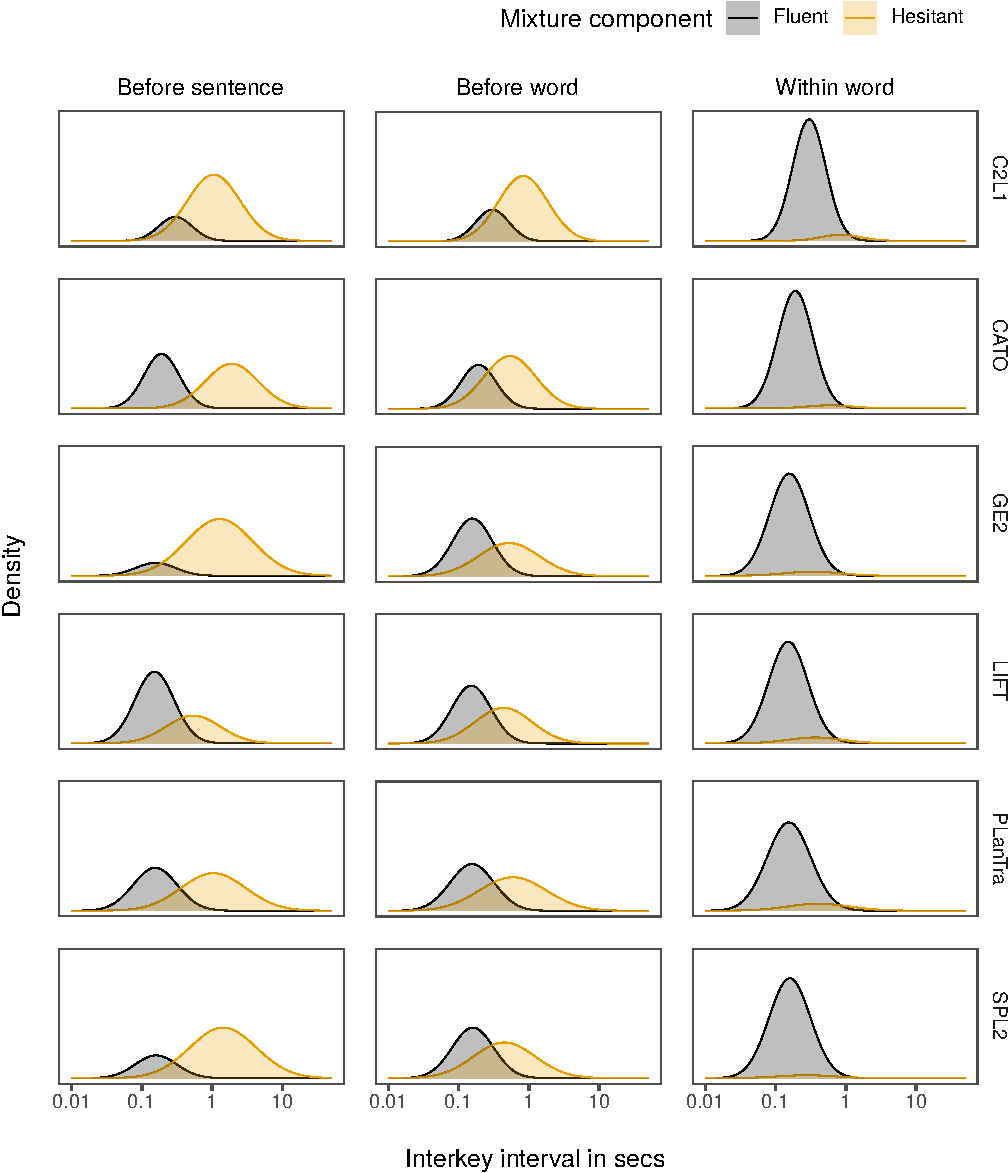
\includegraphics{manuscript_files/figure-latex/mixmodel-1} 

}

\caption{Mixture model plot for each transition location. Shown are the distributions for both mixture components (fluent and hesitant transition durations) and their respective weighting. Posterior of SPL2 data (English sessions only).}\label{fig:mixmodel}
\end{figure}

The predictive performance of the unconstrained mixture model is substantially higher than the predictive performance of the constrained mixture model. However, the constrained mixture model is the theoretically more parsimonious model of the cascading view; in other words, differences between transition locations for the component of fluent transitions were to some extent speculative and unexpected. We therefore present the posterior parameter values for the constrained two-distributions mixture model in the following with reference to the unconstrained implementation.

We present the mixture-model posterior estimates for each of the three parameters in the three facets of Figure \ref{fig:crossstudypost2}. Although models were fitted with all data set-specific condition, we aggregated the posterior across conditions\footnote{We aggregated across pre-post test for the PLanTra dataset as well as genre and topic of the LIFT data set. We demonstrate in Appendix \ref{pre-post-test-plantra} and \ref{genre-effect-lift} respectively that there is negligible evidence of differences between these conditions.}, and removed conditions that might conflate comparisons\footnote{We removed the masked writing condition in the GUNNEXP2 and CATO, the dyslexic group in the CATO data set, and L2 writing in the SPL2 data set. While there was evidence for language-specific effects in Appendix \ref{l2-effect-spl2}, evidence for marking effects was weak as shown in Appendix \ref{masking-effect-cato-gunnexp2}.}. For posteriors of all conditions within data sets see Appendix \ref{posterior-parameter-estimates}. The resulting posterior allows us to examine differences between transition locations for each data set associated with each of the slowdown duration for hesitant transitions and the hesitation probability. Note that the estimate for fluent transitions was estimated by dataset.

\begin{figure}

{\centering 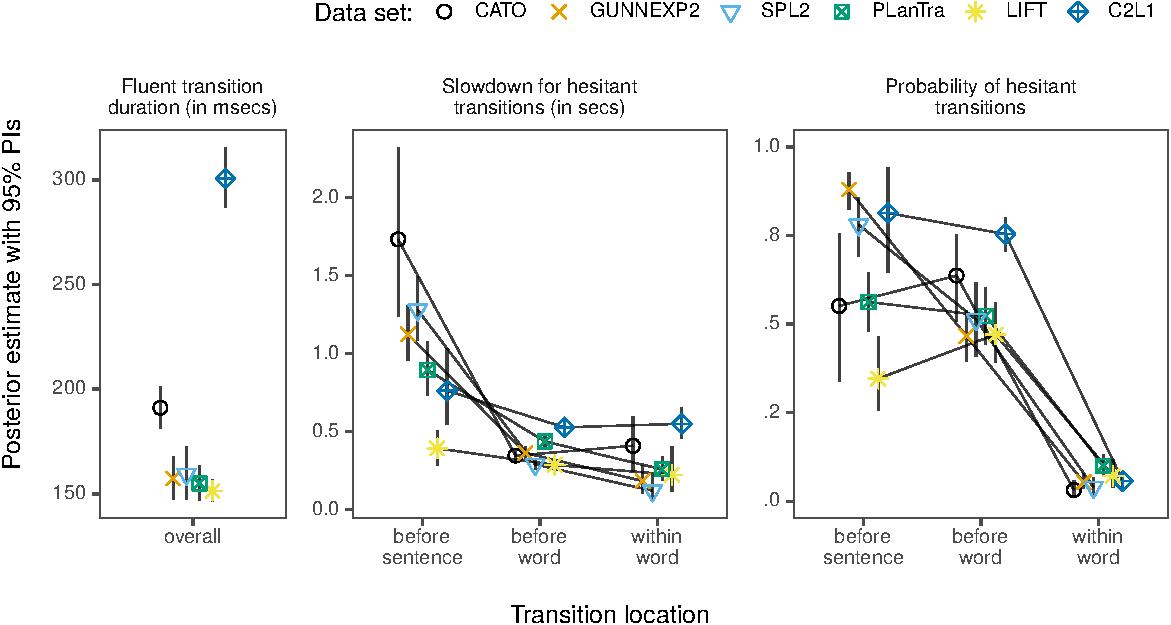
\includegraphics{manuscript_files/figure-latex/crossstudypost2-1} 

}

\caption{Mixture model parameter estimates across studies. Distributions of parameter estimates are represented as posterior mean and 95\% probability interval (PI). Estimates for the CATO dataset were calculated for the non-dyslexic group, unmasked condition; also the GUNNEXP2 estimtes represent the unmasked condition; SPL2 estimates are for the L1 group.}\label{fig:crossstudypost2}
\end{figure}

In the following we evaluate differences between transition locations for all three mixture model parameters. Figure \ref{fig:crossstudypost2} shows largely the same patterns (with caveats) for keystroke-interval estimates by transition location across data sets for all three mixture model parameters. Full results of these pairwise comparisons can be found in Appendix \ref{transition-location-effect-constrained-mixture-model}. We found that hesitations appear more frequently -- higher hesitation probability -- at before-word transitions than within words across data sets (all BFs \textgreater{} 100). Hesitations were more likely at before-sentence locations compared to before-word locations only for 2 out of 6 datasets (GUNNEXP2 and SPL2, both BFs \textgreater{} 100; but C2L1 and CATO: BFs = 0.7; PLanTra: BF = 0.3; LIFT: BF = 1.6). Hesitations were longer at before-sentence transitions compared to before-word transitions (all BFs \textgreater{} 100, except for C2L1: BF = 1.11 and LIFT = 0.5); before-word transitions were longer compared to within-word transitions for half of the data sets (GUNNEXP2: BF = 27; PLanTra: BF = 56; SPL2: BF = 9.1) but not for the other (C2L1: BF = 0.1; CATO: BF = 0.2; LIFT: BF = 0.4).

To reiterate, for most datasets we found negligible evidence supporting the idea that writers pause more frequently at before-sentence boundaries compared to before-word locations (except for datasets SPL2 and GUNNEXP2). This is interesting because it is generally believed that pausing behaviour is associated with syntactic edges such that more and longer pauses are predicted for key transitions at larger syntactic edges following the pattern before-sentence \(>\) before-word \(>\) within-word. In fact, LIFT showed some indication that pauses were less likely before sentences than words. In brief, while pauses tend to be longer before sentences and less likely at mid-word locations, it is less clear in which contexts pauses are (1) longer before than within words and (2) more likely to appear before sentences than before words.

The duration of fluent durations was not distinguished by transition location in the constrained version of the two distribution model. Figure \ref{fig:crossstudypost2} highlights that two datasets (C2L1, CATO) show substantially longer fluent transition durations. This is presumably reflecting that the population that this sample is from was the youngest and least experienced writers in our data pool. Hesitation duration and frequencies were similar to other data sets.

Inconsistencies between datasets could, to some extent, be explained on the basis that before-sentence transitions were sometimes defined as involving complex key combination involve the mean or sum of transitions between space, shift and / or the sentence-initial letters. In particular, before-sentence transitions in some datasets (PLanTra, LIFT) included the character key following the shift key but others did not (CATO, C2L1, SPL2, GUNNEXP2). Appendix \ref{key-combination-effect-constrained-mixture-model} addressed this possibility for the SPL2 dataset and showed that including the character following the shift key substantially increases the hesitation probability (BFs \textgreater{} 100) but it did not affect the duration of fluent transitions or hesitations (BFs \textless{} 0.3). However this is in conflict with the earlier finding that before-sentence hesitations are not more likely than before-word hesitations for the datasets that included the character following shift (PLanTra, LIFT). In other words, it is unlikely that patterns in our results can be explained on the basis of how before-keystroke transitions were operationalised (complex key-combinations at before-sentence locations).

The predictive performance of the unconstrained model was higher compared to the constrained model (see Table \ref{tab:loos}). We, therefore, summarize briefly differences in the results for the transition-location effects. Results for the unconstrained version of the mixture model can be found in Appendix \ref{transition-location-effect-unconstrained-mixture-model}. The main difference between the unconstrained and the constrained model is that the latter does not allow the parameter that captures fluent transition durations to vary by transition location or otherwise. Instead it represents the lower bound of keystroke activity for uninhibited activation flow. Higher predictive performance for the unconstrained model suggests variability across transition locations for fluent transition durations, in particular for before-word transitions compared to mid-word transitions (all BFs \textgreater{} 100) but not for before-sentence transitions compared to before-word transitions (all BFs \textless{} 0.08, but SPL2 and GUNNEXP2: BFs \textgreater{} 100). The pattern for the hesitation probability was generally similar in both the constrained and unconstrained model. However, for hesitation durations the unconstrained model showed evidence for longer durations at before-word locations compared to within-word location in all but one dataset (all BFs \textgreater{} 10, except for LIFT: BF = 0.7); the hesitation duration pattern for before-sentence transitions compared to before-word transitions remained the same.

\hypertarget{discussion}{%
\section{Discussion}\label{discussion}}

The classical serial view (Flower \& Hayes, 1980) characterizes writing as a sequence planning and execution cycles that results in a writing process that consists of bursts interrupted by pauses. Our cascading model of writing, in contrast, captures that planning, at least in competent writers can occur in parallel to production. We used Bayesian statistical models, in particular single-distribution and two-distributions hierarchical models, to directly compare the serial and the cascading model of writing, respectively. On the basis of 6 data sets with key data from free text production tasks, we presented compelling and consistent statistical evidence in favour of the cascading view.

Patters observed in the parameter estimates are generally similar across data sets (with caveats). Under the cascading view of writing, key-transitions that directly precede sentences or words are not necessarily associated with a pause but writers might plan in parallel to writing. On the basis of parameter estimates of the mixture model we tested to what extent larger linguistic edges are associated with the preparation of upcoming planning unit. We found that in 4 of 6 data sets, pauses were as likely to occur before sentences as words, in experienced and novice writers, while mid-word pauses were rare. Also, with few exceptions, pauses at before-sentence locations were associated were longer compared to pauses at before-word transitions (which were longer than the few mid-word pauses). In other words, when writers pause, the duration of their pause generally suggest that larger linguistic edges are associated with higher-level processing. However, the pausing probability results can only be explained by the cascading view of writing, not by the serial view. This is because the hesitation probability results suggest that writers often do not pause before sentences; indeed, they frequently plan the next sentence in parallel production resulting in roughly identical hesitation probabilities at before-sentence and before-word locations.

Interestingly even the youngest sample in our data pool (C2L1) showed evidence of parallel planning. For example, Olive (2014) described a cascading model that is operating in a serial fashion for inexperienced or struggling writers. This is because of task demands reduce the ability to plan in parallel to processing which leads to a separation of planning units that therefore operate in a serial fashion. However, the results presented in this paper suggest that pausing behaviour in young writers largely mirror results from more experienced writers with the notable exception that pause durations are similar before words and sentence indicating a tendency to prepare utterances in small lexically-based planning units possibly smaller than the clause. The main differences for the young writers was their fluent writing execution is substantially slower compared to more experienced writers in the sample. Also for L2 writers (PlanTra, SPL2) we observe pausing patterns that do not resemble a serialised writing process.

We did observe four difference between data sets that are worth highlighting. These can largely be explained on the basis of difference in sample population (writing competence / experience) and text genre (see also Conijn et al., 2019):

First, key-transitions of the youngest sample (C2L1) were substantially longer compared to all other datasets with a larger slowdown before words. Yet the overall pausing probability showed a patterns comparable to most other data sets. In particular, a larger pause probability was observed for transitions before sentences / words compared to mid-word transitions. The second and third exceptions concern the GUNNEXP2 and SPL2 data sets: pauses were more likely to occur at before-sentence transitions compared to before-word transitions while in the remaining data sets hesitations were equally probably at before-word and before-sentence locations (compared to mid-word locations). \textbf{TODO: I don't have an explanation for this.} Also, fluent transitions were longer at before-sentence locations compared to before-word locations while in the remaining data sets fluent key-transitions were always shorter at mid-word compared to before-words transitions. This shows a general tendency to slow down tying at sentence boundaries for the GUNNEXP2 and SPL2 samples which was pronounced in the other data sets. Fourth, pauses were longer before sentence compared to before words compared to mid-word paues with two exceptions: (1) no difference was found for before-sentence compared to before-word transitions in C2L1 possibly due to a a word-level planning strategy in this sample of young writers as inexperienced writers tend to use a more localised strategy for text production. (2) pause durations did not vary by transition location in the LIFT data set although the posterior showed the same general patterns as observed in most data sets. The absence of a difference could be explained as specific to the synthesis writing task {[}\textbf{REFERENCE}{]}.

A possible concern with our results -- substantially better predictive performance for two-distributions mixture models -- is that, in principle, as the mixture model has more parameters it might always lead to a better fit. We addressed this concern by using cross-validation techniques for model comparison which is preventing overfitting models. In addition we used a simulation approach to compare a single distribution model and a two distributions mixture model. We simulated two data sets that were either based on a single distribution or two-distributions random data generating process. In other words, this approach allows us to test the predictive performance of our models in a context where we know the true underlying data generating process -- single distribution vs two-distributions -- and we can test whether these models can successfully uncover the true parameter value. Modelling details can be found in Appendix \ref{simulation}. As might be expected, we found, that the two-distribution mixture was successful at uncovering the parameter values of the data generated with a two-distributions mixture models; we observed the same for the single-distribution model of the data generated with a single distribution process. Parameters were not successfully uncovered when we switched model type and data set. Importantly though, cross-validation did not show a higher predictive performance for the mixture model, compared to the single distribution model, when applied to data based on a two-distributions process (but for the two-distributions data). Therefore we can rule out the possibility that the overwhelming statistical support for the two-distributions mixture models can be explained in terms of model overfitting.

Throughout this paper we assumed that hesitations are indicators of planning upcoming ideas and encoding of linguistic units. Alternatively at least some if not all pauses in the writing process might be the result of reading or looking back into previously produced text. There is a limited amount of work that has used eye tracking to investigate regressive eye movement behaviour during writing (Alamargot et al., 2010; Beers et al., 2010; Chukharev-Hudilainen et al., 2019; De Smet et al., 2018; Torrance et al., n.d.; Van Waes et al., 2010). There are at least three reasons why writers look back into their text: (1) reading is necessary for revision (i.e.~writers must check if writing goals have been met); (2) using text to cue or reinstating ideas after interruption of writing process; (3) error evaluation: e.g.~spelling, grammar. We removed transitions that terminated in an editing operation so the pauses we detected are unlikely to reflect revisions. However, frequencies of lookback during writing follow a similar pattern as the one we observed for pausing: Torrance, Johansson, et al. (2016) reported that lookbacks appear with a frequency of 45\% before sentences, 12\% before words and 5\% within words of which 36\% were associated with sustained reading but mostly less patterned forward and backward saccades between words ({``hopping,''} see also Chukharev-Hudilainen et al., 2019). This is except, look backs are more frequent before sentences compared to words while we found that pause frequencies appear equally often before sentences and words. Finally two of the data sets in our poor (CATO, GUNNEXP2) included a manipulation where the produced text was masked (or not). In a reanalysis we found no substantial differences in pausing behaviour for the masked condition; see Appendix \ref{masking-effect-cato-gunnexp2}. In other words, even though reading is likely be explain some proportion of our results it is overall rare, certainly in samples of university students.

A practical advantage of our mixture model approach (also Roeser et al., 2021) is that we are not required to stipulate interval thresholds as plausible candidate for lower pause bound to handle the complex distribution of latency from spontaneous text production. Such threshold are widely used by writing researchers, a strategy that was inherited from early research in speech production (for review see Rochester, 1973), with studies dating back to at least the mid 1990s (Foulin, 1998). There is one central problems with this approach: A threshold requires a definition of what passes as a pause (Van Waes et al., 2016; Wengelin, 2006), i.e.~a pause criterion threshold often set to 2 secs (Chanquoy et al., 1996; Kaufer et al., 1986; Sullivan \& Lindgren, 2002; Wengelin, 2002) or some other lower bound (Chukharev-Hudilainen, 2014; Connelly et al., 2012; Leijten \& Van Waes, 2013). Even if these thresholds were adjusted relative to factors such as writing medium, experience of writer, and text location of pause (see e.g. Wengelin, 2006) they would be arbitrary. For example, a sentence-initial pause of 2 s has a very different interpretation from a 2 s pause that occurs before or within a word. Our current understanding of the processes that underlie text production does not provide a strong theoretical basis on which to make this decision. So while a 2 secs threshold undoubtedly captures an interesting distinction -- processing that occurs the range zero to 2 secs is very likely to be qualitatively different from processing that takes more than 2 secs. However the same could be argued for any threshold between perhaps 250 msecs and 10 secs that a researcher might care to choose (Chenu et al., 2014). Mixture models provide a principled statistical framework that allows the researcher to model behavioural data that come from a combination of cognitive processes without imposing threshold values (see also Almond et al., 2012; Baaijen et al., 2012; Hall et al., 2022; Li, 2021).

\hypertarget{conclusion}{%
\section{Conclusion}\label{conclusion}}

In contrast to the serial pause-and-burst view, the cascading view emphasis that writers do not necessarily pause to plan the upcoming language unit but plan in parallel to writing execution. Using the Bayesian framework we implemented models of both the serial model of writing and the cascading view. Model comparisons and the inspection of posterior parameter estimates supported with a cascading view of writing but provided strong evidence against the serial view. This pattern was found to be largely consistent different levels of writing experience and languages (e.g.~young / L2 writers, students) and writing tasks (e.g.~essays, syntheses) included in our data pool.

\hypertarget{references}{%
\section{References}\label{references}}

\begingroup
\setlength{\parindent}{-0.5in}
\setlength{\leftskip}{0.5in}

\hypertarget{references}{}

\endgroup

\hypertarget{refs}{}
\begin{CSLReferences}{1}{0}
\leavevmode\hypertarget{ref-ailhaud2018variations}{}%
Ailhaud, E., \& Chenu, F. (2017). Variations of chronometric measures of written production depending on clause packaging. \emph{CogniTextes}, \emph{17}. \url{https://doi.org/10.4000/cognitextes.992}

\leavevmode\hypertarget{ref-ailhaud2016developmental}{}%
Ailhaud, E., Chenu, F., \& Jisa, H. (2016). A developmental perspective on the units of written {F}rench. In J. Perera, M. Aparici, E. Rosado, \& N. Salas (Eds.), \emph{Written and spoken language development across the lifespan: Essays in honour of {Liliana Tolchinsky}} (pp. 287--305). Springer. \url{https://doi.org/10.1007/978-3-319-21136-7_17}

\leavevmode\hypertarget{ref-alamargot2010using}{}%
Alamargot, D., Plane, S., Lambert, E., \& Chesnet, D. (2010). Using eye and pen movements to trace the development of writing expertise: Case studies of a 7th, 9th and 12th grader, graduate student, and professional writer. \emph{Reading and Writing}, \emph{23}(7), 853--888.

\leavevmode\hypertarget{ref-almond2012preliminary}{}%
Almond, R., Deane, P., Quinlan, T., Wagner, M., \& Sydorenko, T. (2012). \emph{A preliminary analysis of keystroke log data from a timed writing task} (Research Report No. RR-12-23). Educational Testing Service.

\leavevmode\hypertarget{ref-alves2015progress}{}%
Alves, R. A., \& Limpo, T. (2015). Progress in written language bursts, pauses, transcription, and written composition across schooling. \emph{Scientific Studies of Reading}, \emph{19}(5), 374--391.

\leavevmode\hypertarget{ref-baaijen2012keystroke}{}%
Baaijen, V. M., Galbraith, D., \& De Glopper, K. (2012). Keystroke analysis: Reflections on procedures and measures. \emph{Written Communication}, \emph{29}(3), 246--277.

\leavevmode\hypertarget{ref-beers2010adolescent}{}%
Beers, S. F., Quinlan, T., \& Harbaugh, A. G. (2010). Adolescent students' reading during writing behaviors and relationships with text quality: An eyetracking study. \emph{Reading and Writing}, \emph{23}(7), 743--775.

\leavevmode\hypertarget{ref-bock2014syntactically}{}%
Bock, J. K., \& Ferreira, V. S. (2014). In M. Goldrick, V. S. Ferreira, \& M. Miozzo (Eds.), \emph{{The Oxford Handbook of Language Production}} (pp. 21--46). Oxford University Press.

\leavevmode\hypertarget{ref-bonin2012evidence}{}%
Bonin, P., Roux, S., Barry, C., \& Canell, L. (2012). Evidence for a limited-cascading account of written word naming. \emph{Journal of Experimental Psychology: Learning, Memory, and Cognition}, \emph{38}(6), 1741--1758. \url{https://doi.org/10.1037/a0028471}

\leavevmode\hypertarget{ref-carpenter2016stan}{}%
Carpenter, B., Gelman, A., Hoffman, M., Lee, D., Goodrich, B., Betancourt, M., Brubaker, M. A., Guo, J., Li, P., \& Riddell, A. (2016). Stan: A probabilistic programming language. \emph{Journal of Statistical Software}, \emph{20}.

\leavevmode\hypertarget{ref-chang2006}{}%
Chang, F., Dell, G. S., \& Bock, J. K. (2006). Becoming syntactic. \emph{Psychological Review}, \emph{113}(2), 234--272.

\leavevmode\hypertarget{ref-chanquoy1996writing}{}%
Chanquoy, L., Foulin, J.-N., \& Fayol, M. (1996). Writing in adults: {A} real-time approach. In G. Rijlaarsdam, H. Van den Bergh, \& M. Couzijn (Eds.), \emph{Theories, models and methodology in writing research} (pp. 36--44). Amsterdam University Press.

\leavevmode\hypertarget{ref-chenoweth2001fluency}{}%
Chenoweth, N. A., \& Hayes, J. R. (2001). Fluency in writing: Generating text in {L1} and {L2}. \emph{Written Communication}, \emph{18}(1), 80--98.

\leavevmode\hypertarget{ref-chenoweth2003inner}{}%
Chenoweth, N. A., \& Hayes, J. R. (2003). The inner voice in writing. \emph{Written Communication}, \emph{20}(1), 99--118.

\leavevmode\hypertarget{ref-chenu2014interword}{}%
Chenu, F., Pellegrino, F., Jisa, H., \& Fayol, M. (2014). Interword and intraword pause threshold in writing. \emph{Frontiers in Psychology}, \emph{5}. \url{https://doi.org/10.3389/fpsyg.2014.00182}

\leavevmode\hypertarget{ref-christiansen2016now}{}%
Christiansen, M. H., \& Chater, N. (2016). The now-or-never bottleneck: A fundamental constraint on language. \emph{Behavioral and Brain Sciences}, \emph{39}, e62. \url{https://doi.org/10.1017/S0140525X1500031X}

\leavevmode\hypertarget{ref-chukharev2014pauses}{}%
Chukharev-Hudilainen, E. (2014). Pauses in spontaneous written communication: {A} keystroke logging study. \emph{Journal of Writing Research}, \emph{6}(1), 61--84.

\leavevmode\hypertarget{ref-chukharev2019combined}{}%
Chukharev-Hudilainen, E., Saricaoglu, A., Torrance, M., \& Feng, H.-H. (2019). Combined deployable keystroke logging and eyetracking for investigating {L2} writing fluency. \emph{Studies in Second Language Acquisition}, \emph{41}(3), 583--604.

\leavevmode\hypertarget{ref-Clark2002}{}%
Clark, H. H., \& Fox Tree, J. E. (2002). Using \emph{uh} and \emph{um} in spontaneous speaking. \emph{Cognition}, \emph{84}, 73--111.

\leavevmode\hypertarget{ref-conijn2020keys}{}%
Conijn, R. (2020). \emph{The keys to writing: A writing analytics approach to studying writing processes using keystroke logging} {[}PhD thesis{]}. Tilburg University.

\leavevmode\hypertarget{ref-conijn2019understanding}{}%
Conijn, R., Roeser, J., \& van Zaanen, M. (2019). Understanding the keystroke log: The effect of writing task on keystroke features. \emph{Reading and Writing}, \emph{32}(9), 2353--2374.

\leavevmode\hypertarget{ref-conijn2021timecourse}{}%
Conijn, R., \& Torrance, M. (Eds.). (2023). Timecourse method. \emph{Reading and Writing}. \url{https://link.springer.com/collections/gedbaiibja}

\leavevmode\hypertarget{ref-connelly2012predicting}{}%
Connelly, V., Dockrell, J. E., Walter, K., \& Critten, S. (2012). Predicting the quality of composition and written language bursts from oral language, spelling, and handwriting skills in children with and without specific language impairment. \emph{Written Communication}, \emph{29}(3), 278--302.

\leavevmode\hypertarget{ref-crump2010hierarchical}{}%
Crump, M. J. C., \& Logan, G. D. (2010). Hierarchical control and skilled typing: Evidence for word-level control over the execution of individual keystrokes. \emph{Journal of Experimental Psychology: Learning, Memory, and Cognition}, \emph{36}(6), 1369--1380. \url{https://doi.org/10.1037/a0020696}

\leavevmode\hypertarget{ref-dam09}{}%
Damian, M. F., \& Stadthagen-Gonzalez, H. (2009). Advance planning of form properties in the written production of single and multiple words. \emph{Language and Cognitive Processes}, \emph{24}(4), 555--579.

\leavevmode\hypertarget{ref-de2018exploring}{}%
De Smet, M. J. R., Leijten, M., \& Van Waes, L. (2018). Exploring the process of reading during writing using eye tracking and keystroke logging. \emph{Written Communication}, \emph{35}(4), 411--447.

\leavevmode\hypertarget{ref-dell2007case}{}%
Dell, G. S., Martin, N., \& Schwartz, M. F. (2007). A case-series test of the interactive two-step model of lexical access: Predicting word repetition from picture naming. \emph{Journal of Memory and Language}, \emph{56}(4), 490--520.

\leavevmode\hypertarget{ref-dux2021effect}{}%
Dux Speltz, E., \& Chukharev-Hudilainen, E. (2021). The effect of automated fluency-focused feedback on text production. \emph{Journal of Writing Research}, \emph{13}(2), 231--255.

\leavevmode\hypertarget{ref-dux2022automating}{}%
Dux Speltz, E., Roeser, J., \& Chukharev-Hudilainen, E. (2022). Automating individualized, process-focused writing instruction: A design-based research study. \emph{Frontiers in Communication: Emerging Technologies and Writing: Pedagogy and Research}, \emph{7}, 933878. \url{https://doi.org/0.3389/fcomm.2022.933878}

\leavevmode\hypertarget{ref-farrell2018computational}{}%
Farrell, S., \& Lewandowsky, S. (2018). \emph{Computational modeling of cognition and behavior}. Cambridge University Press.

\leavevmode\hypertarget{ref-flower1980ynamics}{}%
Flower, L. S., \& Hayes, J. R. (1980). The dynamics of composing: Making plans and juggling constraints. In L. W. Gregg \& E. R. Steinberg (Eds.), \emph{Cognitive processes in writing: An interdisciplinary approach} (pp. 31--50). Lawrence Erlbaum.

\leavevmode\hypertarget{ref-flower1981pregnant}{}%
Flower, L. S., \& Hayes, J. R. (1981). The pregnant pause: An inquiry into the nature of planning. \emph{Research in the Teaching of English}, 229--243.

\leavevmode\hypertarget{ref-foulin1998extent}{}%
Foulin, J.-N. (1998). To what extent does pause location predict pause duration in adults' and children's writing? \emph{Cahiers de Psychologie Cognitive/Current Psychology of Cognition}, \emph{17}, 601--620.

\leavevmode\hypertarget{ref-gelman2014}{}%
Gelman, A., Carlin, J. B., Stern, H. S., Dunson, D. B., Vehtari, A., \& Rubin, D. B. (2014). \emph{Bayesian data analysis} (3rd ed.). Chapman; Hall/CRC.

\leavevmode\hypertarget{ref-gelman1992}{}%
Gelman, A., \& Rubin, D. B. (1992). Inference from iterative simulation using multiple sequences. \emph{Statistical Science}, \emph{7}(4), 457--472.

\leavevmode\hypertarget{ref-gernsbacher1995coherence}{}%
Gernsbacher, M. A., \& Givón, T. (1995). \emph{Coherence in spontaneous text} (Vol. 31). John Benjamins Publishing.

\leavevmode\hypertarget{ref-gri01}{}%
Griffin, Z. M. (2001). Gaze durations during speech reflect word selection and phonological encoding. \emph{Cognition}, \emph{82}(1), B1--B14.

\leavevmode\hypertarget{ref-griffin2003reversed}{}%
Griffin, Z. M. (2003). A reversed word length effect in coordinating the preparation and articulation of words in speaking. \emph{Psychonomic Bulletin \& Review}, \emph{10}(3), 603--609.

\leavevmode\hypertarget{ref-guo2018modeling}{}%
Guo, H., Deane, P. D., van Rijn, P. W., Zhang, M., \& Bennett, R. E. (2018). Modeling basic writing processes from keystroke logs. \emph{Journal of Educational Measurement}, \emph{55}(2), 194--216.

\leavevmode\hypertarget{ref-hall2022constructing}{}%
Hall, S., Baaijen, V. M., \& Galbraith, D. (2022). Constructing theoretically informed measures of pause duration in experimentally manipulated writing. \emph{Reading and Writing}, 1--29.

\leavevmode\hypertarget{ref-hayes2012evidence}{}%
Hayes, J. R. (2012). Evidence from language bursts, revision, and transcription for translation and its relation to other writing processes. In M. Fayol, D. Alamargot, \& V. Berninger (Eds.), \emph{Translation of thought to written text while composing: Advancing theory, knowledge, methods, and applications} (pp. 15--25). Psychology Press.

\leavevmode\hypertarget{ref-jefferys1992ockham}{}%
Jefferys, W. H., \& Berger, J. O. (1992). Ockham's razor and {B}ayesian analysis. \emph{American Scientist}, \emph{80}(1), 64--72.

\leavevmode\hypertarget{ref-kaufer1986composing}{}%
Kaufer, D. S., Hayes, J. R., \& Flower, L. S. (1986). Composing written sentences. \emph{Research in the Teaching of English}, 121--140.

\leavevmode\hypertarget{ref-lambert2018student}{}%
Lambert, B. (2018). \emph{A student's guide to {B}ayesian statistics}. Sage.

\leavevmode\hypertarget{ref-lee13}{}%
Lee, E.-K., Brown-Schmidt, S., \& Watson, D. G. (2013). Ways of looking ahead: Hierarchical planning in language production. \emph{Cognition}, \emph{129}(3), 544--562.

\leavevmode\hypertarget{ref-lee2014bayesian}{}%
Lee, M. D., \& Wagenmakers, E.-J. (2014). \emph{Bayesian cognitive modeling: A practical course}. Cambridge University Press.

\leavevmode\hypertarget{ref-leijten2013keystroke}{}%
Leijten, M., \& Van Waes, L. (2013). Keystroke logging in writing research: Using {Inputlog} to analyze and visualize writing processes. \emph{Written Communication}, \emph{30}(3), 358--392.

\leavevmode\hypertarget{ref-li2021identifying}{}%
Li, T. (2021). Identifying mixture components from large-scale keystroke log data. \emph{Frontiers in Psychology}, \emph{12}, 628660.

\leavevmode\hypertarget{ref-peel2000finite}{}%
MacLahlan, G., \& Peel, D. (2000). \emph{Finite mixture models}. John \& Sons.

\leavevmode\hypertarget{ref-matsuhashi1981pausing}{}%
Matsuhashi, A. (1981). Pausing and planning: The tempo of written discourse production. \emph{Research in the Teaching of English}, 113--134.

\leavevmode\hypertarget{ref-mcelreath2016statistical}{}%
McElreath, R. (2016). \emph{Statistical rethinking: {A} bayesian course with examples in {R} and {Stan}}. CRC Press.

\leavevmode\hypertarget{ref-medimorec2017pauses}{}%
Medimorec, S., \& Risko, E. F. (2017). Pauses in written composition: On the importance of where writers pause. \emph{Reading and Writing}, \emph{30}, 1267--1285.

\leavevmode\hypertarget{ref-medimorec2017disfluency}{}%
Medimorec, S., Young, T. P., \& Risko, E. F. (2017). Disfluency effects on lexical selection. \emph{Cognition}, \emph{158}, 28--32.

\leavevmode\hypertarget{ref-meyer1996}{}%
Meyer, A. S. (1996). Lexical access in phrase and sentence production: Results from picture--word interference experiments. \emph{Journal of Memory and Language}, \emph{35}(4), 477--496.

\leavevmode\hypertarget{ref-mohsen2021second}{}%
Mohsen, M. (2021). Second language learners' pauses over different times intervals in {L2} writing essays: Evidence from a keystroke logging program. \emph{Psycholinguistics}, \emph{30}(1), 180--202. \url{https://doi.org/10.31470/2309-1797-2021-30-1-180-202}

\leavevmode\hypertarget{ref-mohsen2021second}{}%
Mohsen, M. (2021). Second language learners' pauses over different times intervals in {L2} writing essays: Evidence from a keystroke logging program. \emph{Psycholinguistics}, \emph{30}(1), 180--202. \url{https://doi.org/10.31470/2309-1797-2021-30-1-180-202}

\leavevmode\hypertarget{ref-not10}{}%
Nottbusch, G. (2010). Grammatical planning, execution, and control in written sentence production. \emph{Reading and Writing}, \emph{23}(7), 777--801.

\leavevmode\hypertarget{ref-olive2014toward}{}%
Olive, T. (2014). Toward a parallel and cascading model of the writing system: {A} review of research on writing processes coordination. \emph{Journal of Writing Research}, \emph{6}(2), 173--194.

\leavevmode\hypertarget{ref-R-base}{}%
R Core Team. (2020). \emph{R: A language and environment for statistical computing}. R Foundation for Statistical Computing. \url{https://www.R-project.org/}

\leavevmode\hypertarget{ref-rochester1973significance}{}%
Rochester, S. R. (1973). The significance of pauses in spontaneous speech. \emph{Journal of Psycholinguistic Research}, \emph{2}, 51--81.

\leavevmode\hypertarget{ref-roeser2021modelling}{}%
Roeser, J., De Maeyer, S., Leijten, M., \& Van Waes, L. (2021). Modelling typing disfluencies as finite mixture process. \emph{Reading and Writing}, 1--26. \url{https://doi.org/10.1007/s11145-021-10203-z}

\leavevmode\hypertarget{ref-roeser2018advance}{}%
Roeser, J., Torrance, M., \& Baguley, T. (2019). Advance planning in written and spoken sentence production. \emph{Journal of Experimental Psychology: Learning, Memory, and Cognition}, \emph{45}(11), 1983--2009. \url{https://doi.org/10.1037/xlm0000685}

\leavevmode\hypertarget{ref-rossetti2022s}{}%
Rossetti, A., \& Van Waes, L. (2022a). It's not just a phase: Investigating text simplification in a second language from a process and product perspective. \emph{Frontiers in Artificial Intelligence}, \emph{5}. \url{https://doi.org/10.3389/frai.2022.983008}

\leavevmode\hypertarget{ref-rossetti2022text}{}%
Rossetti, A., \& Van Waes, L. (2022b). \emph{Text simplification in second language: Process and product data} {[}Data set{]}. Zenodo. \url{https://doi.org/10.5281/zenodo.6720290}

\leavevmode\hypertarget{ref-roux2013interaction}{}%
Roux, S., McKeeff, T. J., Grosjacques, G., Afonso, O., \& Kandel, S. (2013). The interaction between central and peripheral processes in handwriting production. \emph{Cognition}, \emph{127}(2), 235--241.

\leavevmode\hypertarget{ref-ronneberg2022process}{}%
Rønneberg, V., Torrance, M., Uppstad, P. H., \& Johansson, C. (2022). The process-disruption hypothesis: How spelling and typing skill affects written composition process and product. \emph{Psychological Research}, \emph{86}(7), 2239--2255.

\leavevmode\hypertarget{ref-schilperoord2002cognitive}{}%
Schilperoord, J. (2002). On the cognitive status of pauses in discourse production. In T. Olive \& C. M. Levy (Eds.), \emph{Contemporary tools and techniques for studying writing} (pp. 61--87). Springer.

\leavevmode\hypertarget{ref-schoner2002timing}{}%
Schöner, G. (2002). Timing, clocks, and dynamical systems. \emph{Brain and Cognition}, \emph{48}(1), 31--51.

\leavevmode\hypertarget{ref-sim07}{}%
Simpson, S., \& Torrance, M. (2007). \emph{EyeWrite}. SR Research; Nottingham Trent University.

\leavevmode\hypertarget{ref-sivula2020uncertainty}{}%
Sivula, T., Magnusson, M., Matamoros, A. A., \& Vehtari, A. (2020). Uncertainty in {B}ayesian leave-one-out cross-validation based model comparison. \emph{arXiv Preprint arXiv:2008.10296}.

\leavevmode\hypertarget{ref-rstan}{}%
Stan Development Team. (2018). \emph{{RStan}: The {R} interface to {Stan}}. \url{https://mc-stan.org/}

\leavevmode\hypertarget{ref-sullivan2002self}{}%
Sullivan, K. P. H., \& Lindgren, E. (2002). Self-assessment in autonomous computer-aided second language writing. \emph{ELT Journal}, \emph{56}(3), 258--266.

\leavevmode\hypertarget{ref-torrance201203}{}%
Torrance, M. (2012). EyeWrite -- a tool for recording writers' eye movements. In M. Torrance, D. Alamargot, M. Castelló, F. Ganier, O. Kruse, A. Mangen, L. Tolchinsky, \& L. V. Waes (Eds.), \emph{Learning to write effectively: Current trends in {E}uropean research} (pp. 355--357). Brill. \url{https://doi.org/doi.org/10.1163/9781780529295_082}

\leavevmode\hypertarget{ref-torrance2016reading}{}%
Torrance, M., Johansson, R., Johansson, V., \& Wengelin, Å. (2016). Reading during the composition of multi-sentence texts: An eye-movement study. \emph{Psychological Research}, \emph{80}(5), 729--743.

\leavevmode\hypertarget{ref-torrance2012written}{}%
Torrance, M., \& Nottbusch, G. (2012). Written production of single words and simple sentences. In V. W. Berninger (Ed.), \emph{Past, present, and future contributions of cognitive writing research to cognitive psychology} (pp. 403--422). Psychology Press.

\leavevmode\hypertarget{ref-torrance2018timed}{}%
Torrance, M., Nottbusch, G., Alves, R. A., Arfé, B., Chanquoy, L., Chukharev-Hudilainen, E., Dimakos, I., Fidalgo, R., Hyönä, J., Jóhannesson, Ó. I., \& others. (2018). Timed written picture naming in 14 {E}uropean languages. \emph{Behavior Research Methods}, \emph{50}, 744--758.

\leavevmode\hypertarget{ref-torranceb}{}%
Torrance, M., \& Ofstad, G. (n.d.). \emph{Cascading processes in multi-sentence text production}.

\leavevmode\hypertarget{ref-torrancea}{}%
Torrance, M., Roeser, J., \& Chukharev-Hudilainen, E. (n.d.). \emph{Lookback in {L1 and L2} writing: An eye movement study}.

\leavevmode\hypertarget{ref-torrance2016adolescent}{}%
Torrance, M., Rønneberg, V., Johansson, C., \& Uppstad, P. H. (2016). Adolescent weak decoders writing in a shallow orthography: Process and product. \emph{Scientific Studies of Reading}, \emph{20}(5), 375--388.

\leavevmode\hypertarget{ref-van1991handwriting}{}%
Van Galen, G. P. (1991). Handwriting: Issues for a psychomotor theory. \emph{Human Movement Science}, \emph{10}(2), 165--191.

\leavevmode\hypertarget{ref-van2016keystroke}{}%
Van Waes, L., Leijten, M., Lindgren, E., \& Wengelin, Å. (2016). \emph{Keystroke logging in writing research: Analyzing online writing processes}. 410--426.

\leavevmode\hypertarget{ref-van2019multilingual}{}%
Van Waes, L., Leijten, M., Pauwaert, T., \& Van Horenbeeck, E. (2019). A multilingual copy task: Measuring typing and motor skills in writing with inputlog. \emph{Journal of Open Research Software}, \emph{7}(30), 1--8.

\leavevmode\hypertarget{ref-van2010reading}{}%
Van Waes, L., Leijten, M., \& Quinlan, T. (2010). Reading during sentence composing and error correction: A multilevel analysis of the influences of task complexity. \emph{Reading and Writing}, \emph{23}(7), 803--834.

\leavevmode\hypertarget{ref-waes2019}{}%
Van Waes, L., Leijten, M., Roeser, J., Olive, T., \& Grabowski, J. (2021). Measuring and assessing typing skills in writing research. \emph{Journal of Writing Research}, \emph{13}(1), 107--153. \url{https://doi.org/10.17239/jowr-2021.13.01.04}

\leavevmode\hypertarget{ref-vandermeulen2020mapping}{}%
Vandermeulen, N., De Maeyer, S., Van Steendam, E., Lesterhuis, M., Van den Bergh, H., \& Rijlaarsdam, G. (2020). Mapping synthesis writing in various levels of {Dutch} upper-secondary education: A national baseline study on text quality, writing process and students' perspectives on writing. \emph{Pedagogische Studiën: Tijdschrift Voor Onderwijskunde En Opvoedkunde}, \emph{97}(3), 187--236.

\leavevmode\hypertarget{ref-vandermeulen2020}{}%
Vandermeulen, N., Steendam, E. V., \& Rijlaarsdam, G. (2020). \emph{{DATASET} -- baseline data {LIFT} synthesis writing project} {[}Data set{]}. Zenodo. \url{https://doi.org/10.5281/zenodo.3893538}

\leavevmode\hypertarget{ref-vandermeulen2023writing}{}%
Vandermeulen, N., Van Steendam, E., De Maeyer, S., \& Rijlaarsdam, G. (2023). Writing process feedback based on keystroke logging and comparison with exemplars: Effects on the quality and process of synthesis texts. \emph{Written Communication}, \emph{40}(1), 90--144.

\leavevmode\hypertarget{ref-vasishth2017}{}%
Vasishth, S., Chopin, N., Ryder, R., \& Nicenboim, B. (2017). Modelling dependency completion in sentence comprehension as a {B}ayesian hierarchical mixture process: {A} case study involving {C}hinese relative clauses. \emph{ArXiv e-Prints}.

\leavevmode\hypertarget{ref-vasishth2017feature}{}%
Vasishth, S., Jäger, L. A., \& Nicenboim, B. (2017). Feature overwriting as a finite mixture process: Evidence from comprehension data. \emph{arXiv Preprint arXiv:1703.04081}.

\leavevmode\hypertarget{ref-vehtari2015pareto}{}%
Vehtari, A., Gelman, A., \& Gabry, J. (2015). Pareto smoothed importance sampling. \emph{arXiv Preprint arXiv:1507.02646}.

\leavevmode\hypertarget{ref-vehtari2017practical}{}%
Vehtari, A., Gelman, A., \& Gabry, J. (2017). Practical bayesian model evaluation using leave-one-out cross-validation and {WAIC}. \emph{Statistics and Computing}, \emph{27}(5), 1413--1432.

\leavevmode\hypertarget{ref-wagenmakers2007linear}{}%
Wagenmakers, E.-J., \& Brown, S. (2007). On the linear relation between the mean and the standard deviation of a response time distribution. \emph{Psychological Review}, \emph{114}(3), 830--841. \url{https://doi.org/10.1037/0033-295X.114.3.830}

\leavevmode\hypertarget{ref-wen02}{}%
Wengelin, Å. (2002). \emph{Text production in adults with reading and writing difficulties} {[}PhD thesis{]}. Göteborg University.

\leavevmode\hypertarget{ref-wen06}{}%
Wengelin, Å. (2006). Examining pauses in writing: {T}heory, methods and empirical data. In K. P. H. Sullivan \& E. Lindgren (Eds.), \emph{Computer keystroke logging and writing: Methods and applications} (Vol. 18, pp. 107--130). Elsevier.

\leavevmode\hypertarget{ref-wheeldon_konopka_2023}{}%
Wheeldon, L. R., \& Konopka, A. (2023). \emph{Grammatical encoding for speech production}. Cambridge University Press. \url{https://doi.org/10.1017/9781009264518}

\leavevmode\hypertarget{ref-wheeldon2013}{}%
Wheeldon, L. R., Ohlson, N., Ashby, A., \& Gator, S. (2013). Lexical availability and grammatical encoding scope during spoken sentence production. \emph{The Quarterly Journal of Experimental Psychology}, \emph{66}(8), 1653--1673.

\leavevmode\hypertarget{ref-wing1973response}{}%
Wing, A. M., \& Kristofferson, A. B. (1973). Response delays and the timing of discrete motor responses. \emph{Perception \& Psychophysics}, \emph{14}(1), 5--12.

\end{CSLReferences}


\clearpage
\makeatletter
\efloat@restorefloats
\makeatother


\begin{appendix}
\section{}
\hypertarget{statistical-models}{%
\subsection{Statistical models}\label{statistical-models}}

We are using the Bayesian framework (e.g. Farrell \& Lewandowsky, 2018;
Gelman et al., 2014; Lee \& Wagenmakers, 2014) to implement 5
statistical models of writing and to evaluate which -- the serial or the
cascading view -- captures more successfully the data that arise during
keyboard typing. In other words, we use statistical models to map
between the data and the theoretically assumed process that generates
the data to then compare the predictive power of those models. The
models presented in this section build on one another so that later
model include assumptions of earlier models.

\hypertarget{serial-model-of-writing}{%
\subsubsection{Serial model of writing}\label{serial-model-of-writing}}

\hypertarget{single-distribution-gaussian}{%
\paragraph{Single distribution
Gaussian}\label{single-distribution-gaussian}}

Under the serial view, all planning must be completed priors to the
production onset of the corresponding planning unit. The resulting IKI
is sometimes faster or slower depending on, among others,
psycholinguistic factors. For example, the interval before a word is
shorter for easily retrievable high-frequency words, or longer for low
frequency words, shorter for words with fewer graphemes, syllables, and
morphemes. There are word-specific factors that influence the IKI that
precedes a word but these are beyond the scope of our analysis. We will
capture the variability associated with word-features by assuming that
before-word IKIs can be described as coming from a distribution that is
normal (Gaussian) with two parameters, an unknown mean \(\mu\), that
describes the average IKI associated with word-level planning, and a
standard deviation \(\sigma_\text{e}^2\), that captures the variability
associated with factors that we did not further specify in the model.
This can be expressed as
\(\text{iki}_\text{before word} \sim \text{N}(\mu, \sigma_\text{e}^2)\).
Of importance is the estimated posterior value of \(\mu\) as this value
captures that time it takes to mentally plan a word.

We can extend this simple model of word-planning to other linguistic
location. We introduce earlier that larger linguistic edges are
associated with planning on higher levels. For example, at sentence
boundaries, planning needs to happen for word-level properties -- which
was captured above as average IKI \(\mu\) -- but also higher linguistic
planning such as clause-level meaning, and dependencies of the
sentence-initial noun (Nottbusch et al., 2007; Roeser et al., 2019).
Regression formulas can, and commonly are, used to decompose \(\mu\) and
capture that there is a change in the outcome variable associated with
another factors. We can decompose \(\mu\) as
\(\mu = \alpha + \beta \cdot \text{x}_\text{sentence[0,1]}\) so that
when \(\text{x}_\text{sentence}\) takes on the value 0, the equation
reduces to \(\mu = \alpha\) which is the average IKI for word
boundaries. However when \(\text{x}_\text{sentence}\) takes on the value
1, the average IKI for word boundaries \(\alpha\) is incremented by a
sentence-related slowdown of \(\beta\) msecs. Therefore the value of the
\(\beta\) parameter represents the additional cognitive demand
associated with sentence-initial planning. The application of such a
statistical model to the data will then provide us with an estimate of
the parameter value that can be used for statistical inference
(e.g.~whether there is a statistically meaningful difference between IKI
associated with words and sentences).

For computational ease, we implemented the differences associated with
transition locations as \(\beta_\text{location}\) in equation
\ref{eq:unimodgaus} where \(\text{location}\) is taking on an index for
each transition location. Therefore, the model will return one \(\beta\)
per transition location that capture the posterior distribution of
average IKIs. Also the decomposition of \(\mu\) allows us to address the
fact that some writers are faster than other writers by introducing a
parameter for what is typically called random intercepts
\(u_\text{participant}\). The random intercepts term
\(u_\text{participant}\) is constrained so that the value it takes on
comes from a normal distribution with a mean of 0 and a standard
deviation of \(\sigma_\text{p}^2\). This value is therefore the
difference between the overall posterior estimate and estimate average
IKI of a particular participant (i.e.~a positive value indicates that a
participant is slower than average, a negative value indicates that a
participant is faster than average).

The final model is shown in equation \ref{eq:unimodgaus} and represents
a Gaussian mixed effects model.

\begin{equation}
\begin{aligned}
\label{eq:unimodgaus}
\text{iki}_i \sim\text{ } & \text{N}(\mu_i, \sigma_\text{e}^2)\\
\text{where: } & \mu_i = \beta_\text{location[i]} + u_\text{participant[i]}\\
& u_\text{participant} \sim \text{N}(0, \sigma_\text{p}^2)\\
\text{constraint: } & \sigma_\text{e}^2, \sigma_\text{p}^2>0
\end{aligned}
\end{equation}

Note aside that standard-deviation parameters were constrained to be
positive because standard deviations can never be negative.

\hypertarget{single-distribution-log-gaussian}{%
\paragraph{Single distribution
log-Gaussian}\label{single-distribution-log-gaussian}}

The previous model assumes that the data-generating process is a
Gaussian distribution. The next model is largely identical to the
previous model but instead of assuming a Gaussian, we assume that the
data come from a log-normal (log-Gaussian) distribution. There are, at
least, two arguments for using a log-Gaussian distribution: (1)
log-Gaussians are zero-bound; in contrast to Gaussians, a log-Gaussian
does not allow negative values. IKIs, as the distance between two
subsequent key-down events, must be positive. The lower bound is
delimited by a person's ability to move their fingers and keyboard
polling. (2) the log-scale is known to be a better match for data from
human behaviour and motor responses. In particular, a Gaussian
distribution assumes that units are scaled linearly. For example, a
difference of 25 msecs is the same between 100 and 125 msecs as between
5 secs and 5,025 msecs. This does not necessarily map onto the
psychological interpretation for short and long keyintervals. For
example effects that result on the motor level within words (e.g.~typing
a high vs a low frequency bigram) are smaller than differences that are
due to high levels of processing (retrieving a word in an L1 or L2). In
other words, although an effect of 25 msecs is large in the context
overall fast keyintervals, it is small in the context of overall slow
intervals. Log-Gaussian distributions are a natural way of translating a
linear scale to an exponential scale so that a 25 msecs difference on
the lower end of the IKI scale (motor activity) is more meaningful than
a 25 msecs difference on the upper end of the IKI scale (retrieving
words, planning sentences).

The model can be described as in equation \ref{eq:unimodloggaus} in
which the distribution \(\text{N}()\) was replaced by \(\text{logN}()\).

\begin{equation}
\begin{aligned}
\label{eq:unimodloggaus}
\text{iki}_i \sim\text{ } & \text{logN}(\mu_i, \sigma_\text{e}^2) \\
\text{where: } &
\mu_i = \beta_\text{location[i]} + u_\text{participant[i]}\\
& u_\text{participant} \sim \text{N}(0, \sigma_\text{p}^2) \\
\text{constraint: } & \sigma_\text{e}^2, \sigma_\text{p}^2>0
\end{aligned}
\end{equation}

\hypertarget{single-distribution-unequal-variance-log-gaussian}{%
\paragraph{Single distribution unequal-variance
log-Gaussian}\label{single-distribution-unequal-variance-log-gaussian}}

The third model representing the serial view of writing is a single
distribution unequal-variance model that, except for the
unequal-variance assumption is identical to the model presented in the
previous section. The previous models modelled IKIs as a function of
transition location so that the estimated average IKI depends on the
position of an IKI in the text. The variance associated with the
estimated IKIs for each transition location was assumed to be identical
(equal variance). This assumption is however not in line with what we
know about data from human behaviour. Longer latencies are known to be
associated with a larger variances for both response-time data in
particular (Wagenmakers \& Brown, 2007) and human motor behaviour in
general (Schöner, 2002; Wing \& Kristofferson, 1973). For IKIs pauses at
larger linguistic edges are plausibly associated with a larger variance
because of the larger number of associated processes. Therefore, in
equation \ref{eq:unimoduv}, we introduce the assumption that standard
deviation \(\sigma_{e_\text{location}}^2)\) varies by transition
location.

\begin{equation}
\begin{aligned}
\label{eq:unimoduv}
\text{iki}_i \sim\text{ } & \text{logN}(\mu_i, \sigma_{e_\text{location[i]}}^2) \\
\text{where: } & \mu_i = \beta_\text{location[i]} + u_\text{participant[i]}\\
 & u_\text{participant} \sim \text{N}(0, \sigma_\text{p}^2) \\
 \text{constraint: } & \sigma_\text{e}^2, \sigma_\text{p}^2>0
\end{aligned}
\end{equation}

\hypertarget{parallel-cascading-model-of-writing}{%
\subsubsection{Parallel cascading model of
writing}\label{parallel-cascading-model-of-writing}}

The following two models are are extensions of the models introduced for
the serial view. Crucially, the cascading view allows planning to happen
in parallel to production. Therefore, we will reduce the constrain of
the serial models that requires all planning to be completed before
writing onset. This is done by assuming that IKIs come from a weighted
combination of two distributions.

\hypertarget{two-distributions-log-gaussian-mixture-model-constrained}{%
\paragraph{Two-distributions log-Gaussian mixture model
(constrained)}\label{two-distributions-log-gaussian-mixture-model-constrained}}

This model extends the assumption of the previous model that processing
that involves higher levels of activation lead to longer pauses. Instead
of assuming that there is one process that is shifted for IKIs of larger
linguistic edges, we introduce the assumption that pauses at larger
linguistic edges are more likely but not obligatory. This is achieved by
modelling IKIs as coming from a weighted mixture of two distributions
associated with two different states:

\begin{enumerate}
\def\labelenumi{\arabic{enumi}.}
\item
  Activation can flow into keystrokes without interruption. These fluent
  keystroke transitions are merely constrained by a person's ability to
  move their finger and will be captured by the \(\beta\) parameter in
  equation \ref{eq:bimodcon}. Note that \(\beta\) is represented in both
  log-Gaussian distributions in equation \ref{eq:bimodcon} referring to
  the same unknown parameter.
\item
  Interruptions in the activation flow from higher to lower levels
  result in longer keystroke intervals, when words or their spelling
  could not be retrieved in time. The slowdown for these hesitant
  transitions is captured by \(\delta\) in the first line of equation
  \ref{eq:bimodcon}. The magnitude of the slowdown is associated with
  transition location. This is because delays at larger linguistic units
  are likely to be associated with higher level planning. By
  constraining \(\delta\) to be positive, it captures how much longer
  hesitant IKIs in addition to \(\beta\).
\end{enumerate}

\begin{equation}
\begin{aligned}
\label{eq:bimodcon}
\text{iki}_{i} \sim\text{ } & \theta_\text{location[i], participant[i]} \cdot \text{LogN}(\beta + \delta_\text{location[i]} + u_\text{participant[i]}, \sigma_{e'_\text{location[i]}}^2) + \\
  & (1 - \theta_\text{location[i], participant[i]}) \cdot \text{LogN}(\beta + u_\text{participant[i]}, \sigma_{e_\text{location[i]}}^2)\\
\text{where: } & u_\text{participant} \sim \text{N}(0, \sigma_\text{p}^2) \\
\text{constraint: } & \delta, \sigma_{e}^2, \sigma_\text{e'}^2, \sigma_\text{p}^2>0\\
        & \sigma_{e'}^2 > \sigma_{e}^2\\
        & 0 < \theta < 1
\end{aligned}
\end{equation}

The first line of equation \ref{eq:bimodcon} represents the distribution
of hesitant key transitions, and the second line represents fluent key
transitions. Each of these two distributions is associated with the
mixing weight \(\theta\) which is a proportion that is constrained to be
larger than 0 and smaller than 1. \(\theta\) is here parameterised to
represent the probability that an IKI is associated with the
distribution of long IKIs. This probability is inversely related to the
mixing weight of the distribution of short IKIs by \(1-\theta\) . In
other words, a larger weight of one distribution inevitably means a
lower weight for the other distribution. The weights of both
distributions must sum to 1. We will call this parameter the probability
of hesitant transitions.

The probability of hesitant transitions is assumed to vary as a function
of both transition location and participants. In line with the
literature discussed in the introduction, we assume that pauses are more
likely at larger linguistic edges. As pausing is subject to individual
differences and writing style (skills), we also assume that some
participants pause more at certain transition locations and other
participants pause less. This is akin to what is known as a random
by-participant slopes model.

Lastly, we carried over the unequal variance assumption and let the
standard deviations \(\sigma_{e'}^2\) and \(\sigma_{e}^2\) vary by
transition location. In addition we constrained the variances so that
\(\sigma_{e'}\) associated with the distribution of typing disfluencies
is larger than the variance associated with fluent transitions
\(\sigma_e\) (see Vasishth, Chopin, et al., 2017; Vasishth, Jäger, et
al., 2017). This was achieved by introducing a parameter
\(\sigma_\text{diff}\). The consequence is that fluent transitions are
assumed to come from a narrower distribution than hesitant transitions.

\hypertarget{two-distributions-log-gaussian-mixture-model-unconstrained}{%
\paragraph{Two-distributions log-Gaussian mixture model
(unconstrained)}\label{two-distributions-log-gaussian-mixture-model-unconstrained}}

The size of a fluent key-transition does not necessarily vary by
transition location. In other words, the parameter \(\beta\) is the same
for before-sentence, before-word, and within-word transitions. This is
what we called a constrained model. However, letter bigrams and trigrams
may be systematically executed faster than transitions between between
space and a letter (REFERENCE?) or complex keystrokes that comprise
space and shift-letter combinations for upper case characters before
sentences (we will address the latter possibility in the results
section). This is because bigrams / trigrams might be stored, retrieved
and executed as motor codes but not transitions to a space following a
word or between a space or shift key press preceding a letter. Also,
because of the necessarily larger number of within-word transitions, as
opposed to before-word and sentence transitions, the posterior of the
constrained model is dominated by within-word transition data. We
therefore also implemented an unconstrained model that assumes that the
size of fluent transitions varies across transition locations.

In this model we assume that \(\beta\) varies by transition-location as
illustrated in equation \ref{eq:bimoduncon}.

\begin{equation}
\begin{aligned}
\label{eq:bimoduncon}
\text{iki}_{i} \sim\text{ } & \theta_\text{location[i], participant[i]} \cdot \text{LogN}(\beta_\text{location[i]} + \delta_\text{location[i]} + u_\text{participant[i]}, \sigma_{e'_\text{location[i]}}^2) + \\
  & (1 - \theta_\text{location[i], participant[i]}) \cdot \text{LogN}(\beta_\text{location[i]} + u_\text{participant[i]}, \sigma_{e_\text{location[i]}}^2)\\
    \text{where: }  & u_\text{participant} \sim \text{N}(0, \sigma_\text{p}^2) \\
\text{constraint: } & \delta, \sigma_{e}^2, \sigma_\text{e'}^2, \sigma_\text{p}^2>0\\
        & \sigma_{e'}^2 > \sigma_{e}^2\\
        & 0 < \theta < 1
\end{aligned}
\end{equation}

\hypertarget{refs}{}
\begin{CSLReferences}{1}{0}
\leavevmode\hypertarget{ref-farrell2018computational}{}%
Farrell, S., \& Lewandowsky, S. (2018). \emph{Computational modeling of
cognition and behavior}. Cambridge University Press.

\leavevmode\hypertarget{ref-gelman2014}{}%
Gelman, A., Carlin, J. B., Stern, H. S., Dunson, D. B., Vehtari, A., \&
Rubin, D. B. (2014). \emph{Bayesian data analysis} (3rd ed.). Chapman;
Hall/CRC.

\leavevmode\hypertarget{ref-lee2014bayesian}{}%
Lee, M. D., \& Wagenmakers, E.-J. (2014). \emph{Bayesian cognitive
modeling: A practical course}. Cambridge University Press.

\leavevmode\hypertarget{ref-not07}{}%
Nottbusch, G., Weingarten, R., \& Sahel, S. (2007). From written word to
written sentence production. In M. Torrance, L. van Waes, \& D. W.
Galbraith (Eds.), \emph{Writing and cognition: Research and
applications} (Vol. 20, pp. 31--53). Elsevier.

\leavevmode\hypertarget{ref-roeser2018advance}{}%
Roeser, J., Torrance, M., \& Baguley, T. (2019). Advance planning in
written and spoken sentence production. \emph{Journal of Experimental
Psychology: Learning, Memory, and Cognition}, \emph{45}(11), 1983--2009.
\url{https://doi.org/10.1037/xlm0000685}

\leavevmode\hypertarget{ref-schoner2002timing}{}%
Schöner, G. (2002). Timing, clocks, and dynamical systems. \emph{Brain
and Cognition}, \emph{48}(1), 31--51.

\leavevmode\hypertarget{ref-vasishth2017}{}%
Vasishth, S., Chopin, N., Ryder, R., \& Nicenboim, B. (2017). Modelling
dependency completion in sentence comprehension as a {B}ayesian
hierarchical mixture process: {A} case study involving {C}hinese
relative clauses. \emph{ArXiv e-Prints}.

\leavevmode\hypertarget{ref-vasishth2017feature}{}%
Vasishth, S., Jäger, L. A., \& Nicenboim, B. (2017). Feature overwriting
as a finite mixture process: Evidence from comprehension data.
\emph{arXiv Preprint arXiv:1703.04081}.

\leavevmode\hypertarget{ref-wagenmakers2007linear}{}%
Wagenmakers, E.-J., \& Brown, S. (2007). On the linear relation between
the mean and the standard deviation of a response time distribution.
\emph{Psychological Review}, \emph{114}(3), 830--841.
\url{https://doi.org/10.1037/0033-295X.114.3.830}

\leavevmode\hypertarget{ref-wing1973response}{}%
Wing, A. M., \& Kristofferson, A. B. (1973). Response delays and the
timing of discrete motor responses. \emph{Perception \& Psychophysics},
\emph{14}(1), 5--12.

\end{CSLReferences}
\end{appendix}

\clearpage
\makeatletter
\efloat@restorefloats
\makeatother


\begin{appendix}
\section{}
\hypertarget{fit-to-data}{%
\subsection{Fit to data}\label{fit-to-data}}

Model fit was assessed by testing to what extent simulations obtained
from the model fit the observed data. From each model we obtained 100
simulations (predictions). These can be found in Figure
\ref{fig:prediction}. The model predictions fitted the data
substantially better for the mixture models. The worse fit was observed
for the single distribution Gaussian model which predicted large amounts
of negative keystroke intervals which are implausible. Using a
log-normal distribution removed these negative keystroke intervals.

\begin{figure}

{\centering 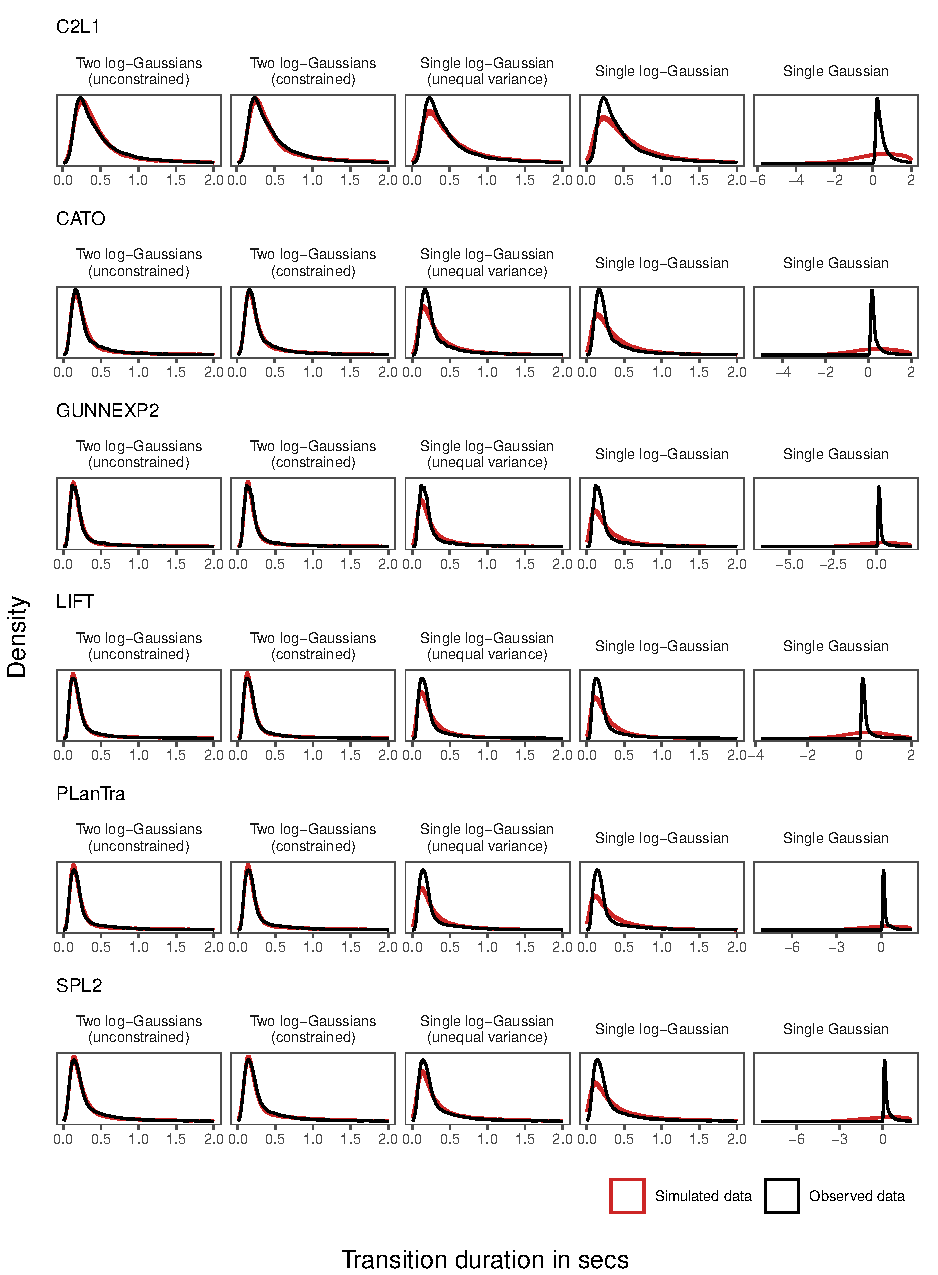
\includegraphics{figures/fitplots} 

}

\caption{Fit to data with models (distribution type) above the plots. Comparison of 50 simulations to observed data summarised by model. For illustration the x-axis was truncated at 2 secs.}\label{fig:prediction}
\end{figure}
\end{appendix}

\clearpage
\makeatletter
\efloat@restorefloats
\makeatother


\begin{appendix}
\section{}
\hypertarget{posterior-parameter-estimates}{%
\subsection{Posterior parameter
estimates}\label{posterior-parameter-estimates}}

\begin{figure}[!htb]
\centering
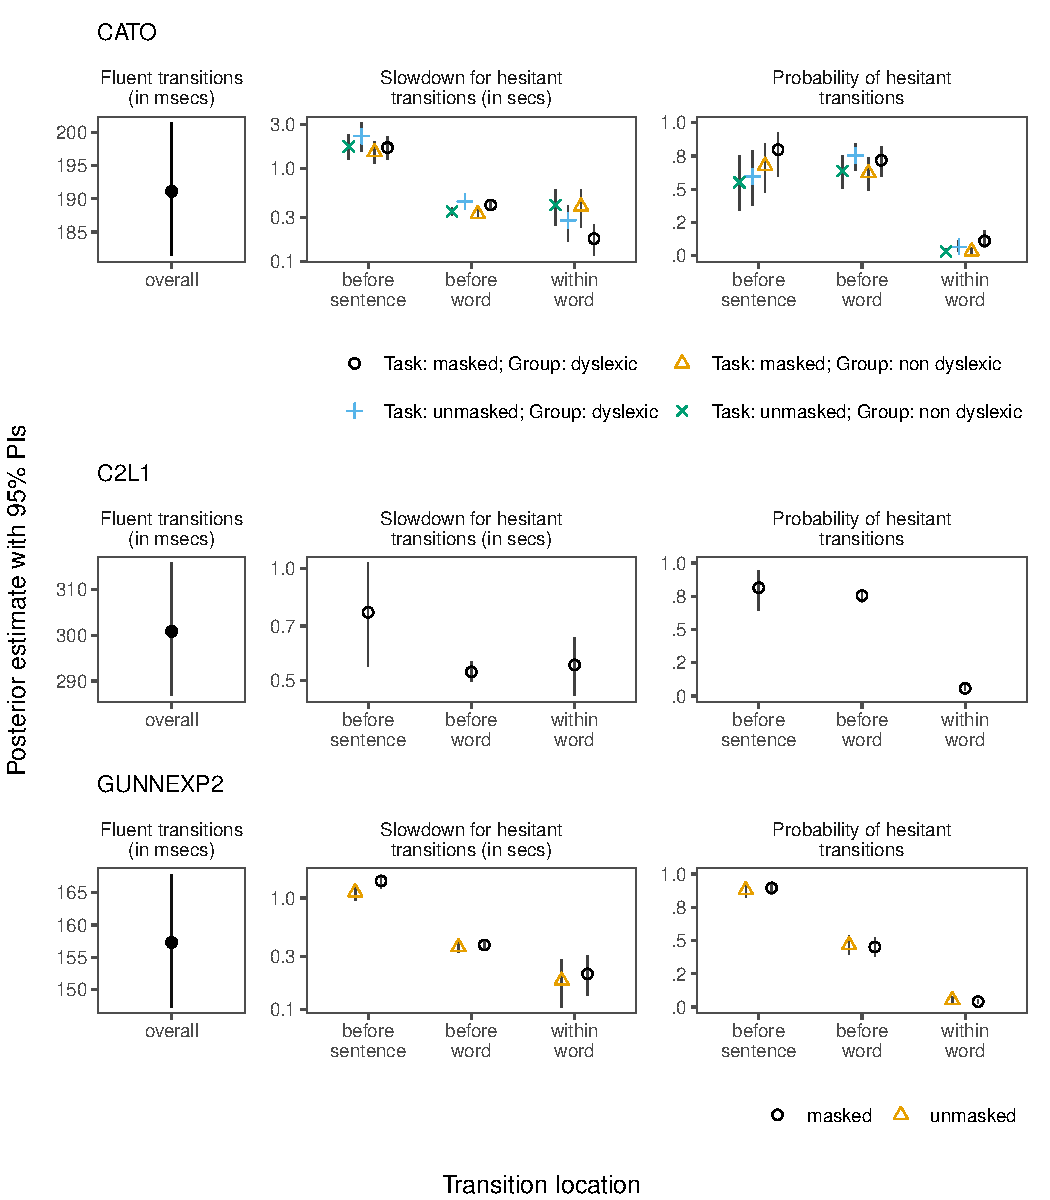
\includegraphics{figures/psplots1constr.pdf}
\caption{Posterior parameter distribution}
\end{figure}
\newpage
\begin{figure}[!htb]
\ContinuedFloat
\captionsetup{list=off,format=cont}
\centering
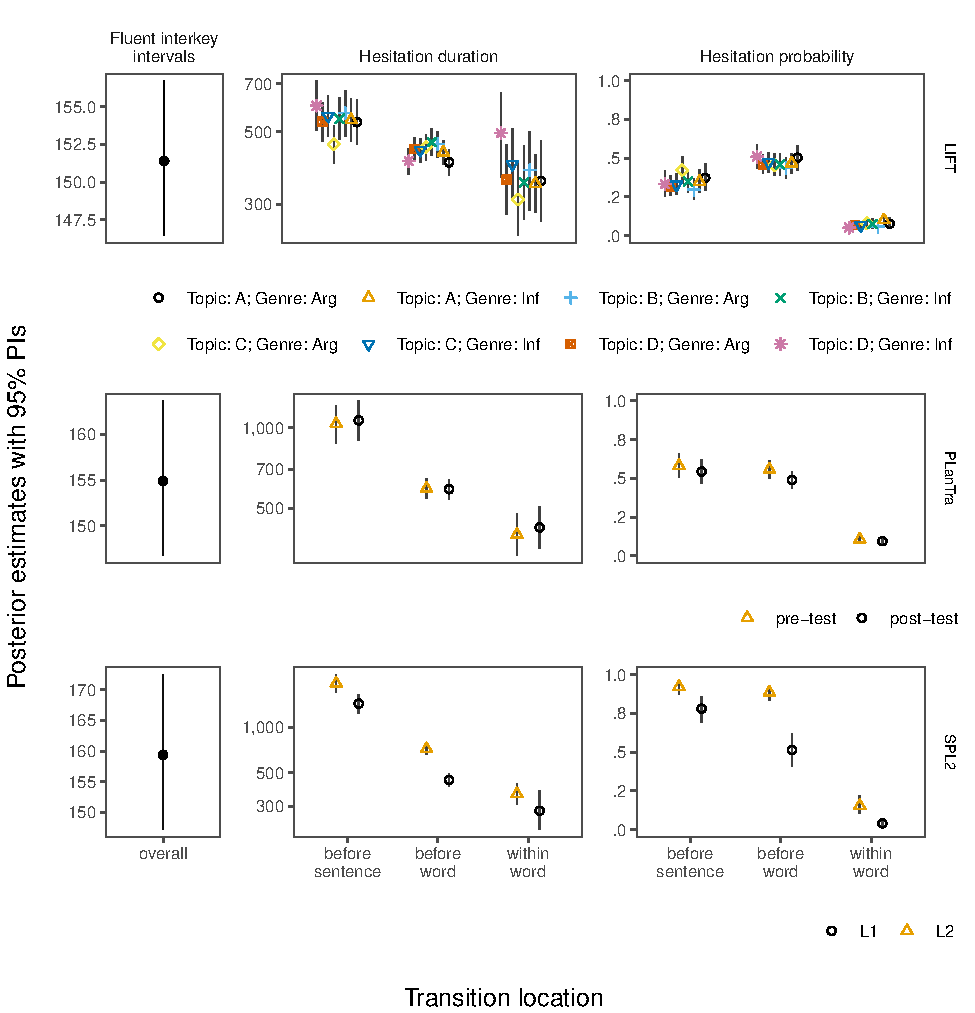
\includegraphics{figures/psplots2constr.pdf}
\label{fig:fullps1}
\caption{Posterior parameter distribution}
\end{figure}
\end{appendix}

\clearpage
\makeatletter
\efloat@restorefloats
\makeatother


\begin{appendix}
\section{}
\hypertarget{key-combination-effect-constrained-mixture-model}{%
\subsection{Key-combination effect (constrained mixture
model)}\label{key-combination-effect-constrained-mixture-model}}

The analysed datasets differ to the extent that keystroke intervals at
before sentence location sometimes did (PLanTra, LIFT) or did not (CATO,
C2L1, SPL2, GUNNEXP2) scope over the character following the shift key.
In other words, the pause before sentences summed across two key
intervals in the PLanTra and LIFT data, namely
\texttt{\_\^{}{[}shift{]}\^{}C} but only involved one key interval,
namely \texttt{\_\^{}{[}shift{]}} for the remaining datasets. Therefore,
longer or more frequent pauses at before-sentence locations compared to
before-word locations can be explained without reference to linguistic
edges.

Therefore we compared whether the different patterns can be explain on
the basis of the additional keystroke involved in before-sentence
transitions. We compared the SPL2 data including and excluding the
keystroke after shift. Although we modelled all transition locations, we
present only before-sentence transitions below as there was, as one
would expect, no difference at word locations. The results of this
comparison can be found in Table \ref{tab:shiftcellmeans}.

\begin{center}
\begin{ThreePartTable}

\begin{TableNotes}[para]
\normalsize{\textit{Note.} PIs are probability intervals. BF is the evidence in favour of the alternative hypothesis over the null hypothesis.}
\end{TableNotes}

\footnotesize{

\begin{longtable}{lrrrr}\noalign{\getlongtablewidth\global\LTcapwidth=\longtablewidth}
\caption{\label{tab:shiftcellmeans}Mixture model estimates for key transitions immediately preceding a sentence. Cell means are shown for transitions that do and do not involve the transition to the character following shift in msecs for the slowdown for long transitions and the probability of hesitant transitions. The difference for including the transition duration to the character after shift is shown on log scale (for transition durations) and logit scale for probability of hesitant transitions. 95\% PIs in brackets.}\\
\toprule
Language & \multicolumn{1}{c}{\_\textasciicircum{}[shift] + C} & \multicolumn{1}{c}{\_\textasciicircum{}[shift]} & \multicolumn{1}{c}{Difference} & \multicolumn{1}{c}{BF}\\
\midrule
\endfirsthead
\caption*{\normalfont{Table \ref{tab:shiftcellmeans} continued}}\\
\toprule
Language & \multicolumn{1}{c}{\_\textasciicircum{}[shift] + C} & \multicolumn{1}{c}{\_\textasciicircum{}[shift]} & \multicolumn{1}{c}{Difference} & \multicolumn{1}{c}{BF}\\
\midrule
\endhead
Fluent transitions &  &  &  & \\
\ \ \ overall & 156 [145, 169] & 159 [147, 172] & -0.02 [-0.13, 0.09] & 0.06\\
Hesitation duration &  &  &  & \\
\ \ \ L1 & 1,167 [1,037, 1,305] & 1,281 [1,082, 1,496] & -0.06 [-0.21, 0.09] & 0.11\\
\ \ \ L2 & 2,019 [1,772, 2,292] & 1,802 [1,557, 2,073] & 0.12 [-0.02, 0.27] & 0.29\\
Hesitation probability &  &  &  & \\
\ \ \ L1 & 1.00 [.99, 1.00] & .78 [.69, .86] & 4.91 [3.68, 6.35] & > 100\\
\ \ \ L2 & 1.00 [.99, 1.00] & .92 [.87, .96] & 3.4 [2.12, 4.85] & > 100\\
\bottomrule
\addlinespace
\insertTableNotes
\end{longtable}

}

\end{ThreePartTable}
\end{center}

The fluent transition duration and hesitation duration were not affected
by whether or not the sentence-initial transition include the character
following shift for neither language. However, we found strong evidence
for an increased hesitation probability -- in both -- languages when the
before-sentence key transition included the character following the
shift key. Notably, the hesitation probability increased ceiling. It is
not entirely surprised that the constrained mixture model identifies
essentially all before-sentence transition as pauses: the constrained
model does not distinguish between transition locations for the duration
of fluent transitions. Therefore essentially all before-sentence
transitions are identified as hesitation as they always include two
keystrokes while all other transition location (which is the majority of
the data) do not.
\end{appendix}

\clearpage
\makeatletter
\efloat@restorefloats
\makeatother


\begin{appendix}
\section{}
\hypertarget{l2-effect-spl2}{%
\subsection{L2 effect (SPL2)}\label{l2-effect-spl2}}

For the SPL2 data (only the \texttt{\_\^{}{[}shift{]}}
sentence-transitions) we calculated the L2 effect (i.e.~the difference
between writing in L2 and L1). The results can be found in Table
\ref{tab:l2effect}. The results show longer hesitation duration and more
pauses across all transition locations when writing in L2. Only
within-word transitions did show negligible evidence for an increased
hesitation duration in L2.

\begin{table}[b]

\begin{center}
\begin{threeparttable}

\caption{\label{tab:l2effect}Mixture model estimates for language effect. Cell means are shown the slowdown for hesitant transitions when writing in L1 and L2 and the probability of hesitant transitions. The language difference is shown on log scale (for transition durations) and logit scale for probability of hesitant transitions. 95\% PIs in brackets.}

\small{

\begin{tabular}{lrrrr}
\toprule
Transition location & \multicolumn{1}{c}{L1} & \multicolumn{1}{c}{L2} & \multicolumn{1}{c}{Difference} & \multicolumn{1}{c}{BF}\\
\midrule
Hesitation duration &  &  &  & \\
\ \ \ before sentence & 1,281 [1,082, 1,496] & 1,802 [1,557, 2,073] & 0.31 [0.17, 0.45] & > 100\\
\ \ \ before word & 289 [254, 327] & 560 [507, 617] & 0.47 [0.39, 0.55] & > 100\\
\ \ \ within word & 120 [53, 222] & 202 [156, 258] & 0.27 [-0.07, 0.55] & 0.68\\
Hesitation probability &  &  &  & \\
\ \ \ before sentence & .78 [.69, .86] & .92 [.87, .96] & 1.23 [0.52, 1.97] & > 100\\
\ \ \ before word & .51 [.41, .62] & .89 [.83, .93] & 2.02 [1.4, 2.66] & > 100\\
\ \ \ within word & .04 [.02, .07] & .15 [.10, .22] & 1.52 [0.78, 2.29] & > 100\\
\bottomrule
\addlinespace
\end{tabular}

}

\begin{tablenotes}[para]
\normalsize{\textit{Note.} PIs are probability intervals. BF is the evidence in favour of the alternative hypothesis over the null hypothesis.}
\end{tablenotes}

\end{threeparttable}
\end{center}

\end{table}
\end{appendix}

\clearpage
\makeatletter
\efloat@restorefloats
\makeatother


\begin{appendix}
\section{}
\hypertarget{masking-effect-cato-gunnexp2}{%
\subsection{Masking effect (CATO,
GUNNEXP2)}\label{masking-effect-cato-gunnexp2}}

Studies associated with two datasets (CATO, GUNNEXP2) investigated to
what extent masking the previously written text affects keystroke
behaviour. The mixture model results for the effect of masking is shown
in Table \ref{tab:maskingeffect}. There was some evidence for longer
before-sentence hesitation durations when the text was masked in
non-dyslexic writers. Evidence for all other comparisons was negligible.

\blandscape

\begin{center}
\begin{ThreePartTable}

\begin{TableNotes}[para]
\normalsize{\textit{Note.} PIs are probability intervals. BF is the evidence in favour of the alternative hypothesis over the null hypothesis.}
\end{TableNotes}

\footnotesize{

\begin{longtable}{lllrrrr}\noalign{\getlongtablewidth\global\LTcapwidth=\longtablewidth}
\caption{\label{tab:maskingeffect}Mixture model estimates for masking effect. Cell means are shown for the masked and unmasked writing task in msecs for the slowdown for long transitions and the probability of hesitant transitions. The effect for masking is shown on log scale (for transition durations) and logit scale for probability of hesitant transitions. 95\% PIs in brackets.}\\
\toprule
Transition location & \multicolumn{1}{c}{Dataset} & \multicolumn{1}{c}{Group} & \multicolumn{1}{c}{Unmasked} & \multicolumn{1}{c}{Masked} & \multicolumn{1}{c}{Difference} & \multicolumn{1}{c}{BF}\\
\midrule
\endfirsthead
\caption*{\normalfont{Table \ref{tab:maskingeffect} continued}}\\
\toprule
Transition location & \multicolumn{1}{c}{Dataset} & \multicolumn{1}{c}{Group} & \multicolumn{1}{c}{Unmasked} & \multicolumn{1}{c}{Masked} & \multicolumn{1}{c}{Difference} & \multicolumn{1}{c}{BF}\\
\midrule
\endhead
Hesitation duration &  &  &  &  &  & \\
\ \ \ before sentence & CATO & dyslexic & 2,231 [1,543, 3,111] & 1,680 [1,239, 2,205] & -0.25 [-0.64, 0.13] & 0.44\\
\ \ \ before sentence & CATO & non dyslexic & 1,733 [1,241, 2,325] & 1,502 [1,134, 1,942] & -0.12 [-0.47, 0.22] & 0.23\\
\ \ \ before sentence & GUNNEXP2 & non dyslexic & 1,124 [954, 1,307] & 1,418 [1,218, 1,634] & 0.21 [0.05, 0.36] & 2.59\\
\ \ \ before word & CATO & dyslexic & 444 [405, 485] & 407 [369, 447] & -0.06 [-0.13, 0.01] & 0.14\\
\ \ \ before word & CATO & non dyslexic & 345 [312, 381] & 326 [295, 361] & -0.04 [-0.11, 0.04] & 0.06\\
\ \ \ before word & GUNNEXP2 & non dyslexic & 363 [325, 403] & 379 [341, 420] & 0.03 [-0.05, 0.11] & 0.05\\
\ \ \ within word & CATO & dyslexic & 278 [166, 400] & 177 [116, 252] & -0.24 [-0.52, 0.06] & 0.57\\
\ \ \ within word & CATO & non dyslexic & 409 [244, 593] & 392 [230, 591] & -0.03 [-0.42, 0.38] & 0.2\\
\ \ \ within word & GUNNEXP2 & non dyslexic & 182 [105, 279] & 209 [135, 306] & 0.08 [-0.24, 0.4] & 0.19\\
Hesitattion probability &  &  &  &  &  & \\
\ \ \ before sentence & CATO & dyslexic & .60 [.38, .79] & .80 [.60, .93] & 0.2 [-0.06, 0.46] & 0.45\\
\ \ \ before sentence & CATO & non dyslexic & .55 [.34, .76] & .68 [.47, .84] & 0.13 [-0.16, 0.4] & 0.21\\
\ \ \ before sentence & GUNNEXP2 & non dyslexic & .88 [.82, .93] & .90 [.85, .94] & 0.16 [-0.46, 0.79] & 0.36\\
\ \ \ before word & CATO & dyslexic & .75 [.64, .85] & .72 [.59, .82] & -0.04 [-0.19, 0.12] & 0.09\\
\ \ \ before word & CATO & non dyslexic & .64 [.51, .75] & .62 [.49, .74] & -0.02 [-0.19, 0.16] & 0.09\\
\ \ \ before word & GUNNEXP2 & non dyslexic & .47 [.40, .54] & .45 [.38, .52] & -0.06 [-0.46, 0.35] & 0.21\\
\ \ \ within word & CATO & dyslexic & .07 [.03, .12] & .11 [.06, .19] & 0.05 [-0.02, 0.13] & 0.08\\
\ \ \ within word & CATO & non dyslexic & .03 [.02, .06] & .03 [.02, .06] & 0 [-0.03, 0.03] & 0.01\\
\ \ \ within word & GUNNEXP2 & non dyslexic & .05 [.03, .08] & .04 [.03, .06] & -0.29 [-0.88, 0.28] & 0.48\\
\bottomrule
\addlinespace
\insertTableNotes
\end{longtable}

}

\end{ThreePartTable}
\end{center}
\elandscape
\end{appendix}

\clearpage
\makeatletter
\efloat@restorefloats
\makeatother


\begin{appendix}
\section{}
\hypertarget{pre-post-test-plantra}{%
\subsection{Pre-post test (PLanTra)}\label{pre-post-test-plantra}}

The pre-post test effect for the PLanTra dataset is reported in Table
\ref{tab:retesteffect}. Evidence for all comparisons was negligible.

\begin{center}
\begin{ThreePartTable}

\begin{TableNotes}[para]
\normalsize{\textit{Note.} PIs are probability intervals. BF is the evidence in favour of the alternative hypothesis over the null hypothesis.}
\end{TableNotes}

\footnotesize{

\begin{longtable}{lrrrr}\noalign{\getlongtablewidth\global\LTcapwidth=\longtablewidth}
\caption{\label{tab:retesteffect}Mixture model estimates for post-test effect. Cell means are shown for the pre-test and post-test in msecs for the slowdown for hesitant transitions and the probability of hesitant transitions. The effect for post-test is shown on log scale (for transition durations) and logit scale for probability of hesitant transitions. 95\% PIs in brackets.}\\
\toprule
Transition location & \multicolumn{1}{c}{Pre-test} & \multicolumn{1}{c}{Post-test} & \multicolumn{1}{c}{Difference} & \multicolumn{1}{c}{BF}\\
\midrule
\endfirsthead
\caption*{\normalfont{Table \ref{tab:retesteffect} continued}}\\
\toprule
Transition location & \multicolumn{1}{c}{Pre-test} & \multicolumn{1}{c}{Post-test} & \multicolumn{1}{c}{Difference} & \multicolumn{1}{c}{BF}\\
\midrule
\endhead
Hesitation duration &  &  &  & \\
\ \ \ before sentence & 879 [723, 1,052] & 909 [740, 1,100] & -0.03 [-0.23, 0.17] & 0.1\\
\ \ \ before word & 438 [395, 485] & 434 [389, 483] & 0.01 [-0.08, 0.1] & 0.05\\
\ \ \ within word & 245 [180, 323] & 269 [201, 353] & -0.06 [-0.3, 0.18] & 0.14\\
Hesitation probability &  &  &  & \\
\ \ \ before sentence & .58 [.50, .66] & .54 [.47, .62] & 0.15 [-0.26, 0.58] & 0.27\\
\ \ \ before word & .56 [.50, .61] & .49 [.43, .55] & 0.27 [-0.04, 0.59] & 0.72\\
\ \ \ within word & .11 [.08, .14] & .09 [.07, .12] & 0.13 [-0.27, 0.54] & 0.26\\
\bottomrule
\addlinespace
\insertTableNotes
\end{longtable}

}

\end{ThreePartTable}
\end{center}
\end{appendix}

\clearpage
\makeatletter
\efloat@restorefloats
\makeatother


\begin{appendix}
\section{}
\hypertarget{genre-effect-lift}{%
\subsection{Genre effect (LIFT)}\label{genre-effect-lift}}

From the LIFT data, we compared the difference between genres, i.e.~when
writing an informative text as opposed to writing an argumentative text.
The results are shown in Table \ref{tab:genreeffect}. Cellmeans and
differences were average across writing topic. Evidence for a genre
comparisons was negligible.

\begin{center}
\begin{ThreePartTable}

\begin{TableNotes}[para]
\normalsize{\textit{Note.} PIs are probability intervals. BF is the evidence in favour of the alternative hypothesis over the null hypothesis.}
\end{TableNotes}

\footnotesize{

\begin{longtable}{lrrrr}\noalign{\getlongtablewidth\global\LTcapwidth=\longtablewidth}
\caption{\label{tab:genreeffect}Mixture model estimates for genre effect. Cell means are shown for argumentative and informative texts in msecs for the hesitation slowdown and the probability of hesitant transitions. The effect for genre is shown on log scale (for transition durations) and logit scale for probability of hesitant transitions. 95\% PIs in brackets.}\\
\toprule
Transition location & \multicolumn{1}{c}{Argumentative} & \multicolumn{1}{c}{Informative} & \multicolumn{1}{c}{Difference} & \multicolumn{1}{c}{BF}\\
\midrule
\endfirsthead
\caption*{\normalfont{Table \ref{tab:genreeffect} continued}}\\
\toprule
Transition location & \multicolumn{1}{c}{Argumentative} & \multicolumn{1}{c}{Informative} & \multicolumn{1}{c}{Difference} & \multicolumn{1}{c}{BF}\\
\midrule
\endhead
Hesitation duration &  &  &  & \\
\ \ \ before sentence & 373 [301, 454] & 411 [330, 504] & -0.07 [-0.33, 0.19] & 0.16\\
\ \ \ before word & 287 [250, 326] & 284 [248, 323] & 0.01 [-0.15, 0.16] & 0.09\\
\ \ \ within word & 199 [118, 306] & 246 [155, 361] & -0.12 [-0.6, 0.36] & 0.29\\
Hesitation probability &  &  &  & \\
\ \ \ before sentence & .35 [.28, .43] & .34 [.27, .42] & 0.05 [-0.57, 0.73] & 0.36\\
\ \ \ before word & .46 [.39, .54] & .48 [.41, .55] & -0.05 [-0.51, 0.44] & 0.25\\
\ \ \ within word & .07 [.05, .10] & .07 [.05, .10] & -0.02 [-0.81, 0.76] & 0.46\\
\bottomrule
\addlinespace
\insertTableNotes
\end{longtable}

}

\end{ThreePartTable}
\end{center}
\end{appendix}

\clearpage
\makeatletter
\efloat@restorefloats
\makeatother


\begin{appendix}
\section{}
\hypertarget{transition-location-effect-constrained-mixture-model}{%
\subsection{Transition location effect (constrained mixture
model)}\label{transition-location-effect-constrained-mixture-model}}

\begin{center}
\begin{ThreePartTable}

\begin{TableNotes}[para]
\normalsize{\textit{Note.} PI = probability intervals. BF = evidence in favour of the alternative hypothesis over the null hypothesis.}
\end{TableNotes}

\footnotesize{

\begin{longtable}{lrrrr}\noalign{\getlongtablewidth\global\LTcapwidth=\longtablewidth}
\caption{\label{tab:loceffectcon}Effect of transition location on keystroke intervals. Differences are shown on log scale (for durations) and logit scale for hesitation probability. 95\% PIs in brackets.}\\
\toprule
 \multicolumn{1}{c}{ } & \multicolumn{2}{c}{Hesitation slowdown} & \multicolumn{2}{c}{Hesitation probability} \\
\cmidrule(r){1-1} \cmidrule(r){2-3} \cmidrule(r){4-5}
Comparison & Est. [95\% PIs] & BF & Est. [95\% PIs] & BF\\
\midrule
\endfirsthead
\caption*{\normalfont{Table \ref{tab:loceffectcon} continued}}\\
\toprule
 \multicolumn{1}{c}{ } & \multicolumn{2}{c}{Hesitation slowdown} & \multicolumn{2}{c}{Hesitation probability} \\
\cmidrule(r){1-1} \cmidrule(r){2-3} \cmidrule(r){4-5}
Comparison & Est. [95\% PIs] & BF & Est. [95\% PIs] & BF\\
\midrule
\endhead
\textbf{C2L1} &  &  &  & \\
\ \ \ before sentence vs word & 0.24 [0.02, 0.48] & 1.11 & 0.44 [-0.56, 1.66] & 0.68\\
\ \ \ before vs within word & -0.03 [-0.14, 0.09] & 0.07 & 3.95 [3.54, 4.38] & > 100\\
\textbf{CATO (non-dyslexic, unmasked)} &  &  &  & \\
\ \ \ before sentence vs word & 1.27 [0.98, 1.55] & > 100 & -0.36 [-1.41, 0.69] & 0.67\\
\ \ \ before vs within word & -0.1 [-0.38, 0.21] & 0.2 & 4.05 [3.2, 4.91] & > 100\\
\textbf{GUNNEXP2 (unmasked)} &  &  &  & \\
\ \ \ before sentence vs word & 0.9 [0.76, 1.04] & > 100 & 2.15 [1.6, 2.75] & > 100\\
\ \ \ before vs within word & 0.44 [0.17, 0.69] & 26.78 & 2.76 [2.24, 3.28] & > 100\\
\textbf{LIFT} &  &  &  & \\
\ \ \ before sentence vs word & 0.21 [-0.05, 0.48] & 0.5 & -0.53 [-1.04, 0.08] & 1.61\\
\ \ \ before vs within word & 0.17 [-0.32, 0.53] & 0.41 & 2.48 [1.81, 3.22] & > 100\\
\textbf{PLanTra} &  &  &  & \\
\ \ \ before sentence vs word & 0.57 [0.4, 0.74] & > 100 & 0.16 [-0.25, 0.57] & 0.28\\
\ \ \ before vs within word & 0.36 [0.16, 0.56] & 55.53 & 2.3 [1.9, 2.7] & > 100\\
\textbf{SPL2 (L1)} &  &  &  & \\
\ \ \ before sentence vs word & 1.17 [1.02, 1.3] & > 100 & 1.23 [0.59, 1.88] & > 100\\
\ \ \ before vs within word & 0.48 [0.16, 0.76] & 9.07 & 3.3 [2.56, 4.08] & > 100\\
\bottomrule
\addlinespace
\insertTableNotes
\end{longtable}

}

\end{ThreePartTable}
\end{center}
\end{appendix}

\clearpage
\makeatletter
\efloat@restorefloats
\makeatother


\begin{appendix}
\section{}
\hypertarget{transition-location-effect-unconstrained-mixture-model}{%
\subsection{Transition location effect (unconstrained mixture
model)}\label{transition-location-effect-unconstrained-mixture-model}}

We present the mixture-model posterior estimates for each of the three
parameter values in the three facets of Figure \ref{fig:crossstudypost}.
Similar to the constrained mixture model, we aggregated the posterior
across conditions\footnote{We aggregated across pre-post test for the
  PLanTra dataset as well as genre and topic of the LIFT data set.} and
removed conditions that might conflate comparisons\footnote{We removed
  the masked writing condition in the GUNNEXP2 and CATO, the dyslexic
  group in the CATO data set, and L2 writing in the SPL2 data set.}. The
resulting posterior allows us to examine differences between transition
locations for each data set associated with each of the three
mixture-model parameters.

\begin{figure}

{\centering 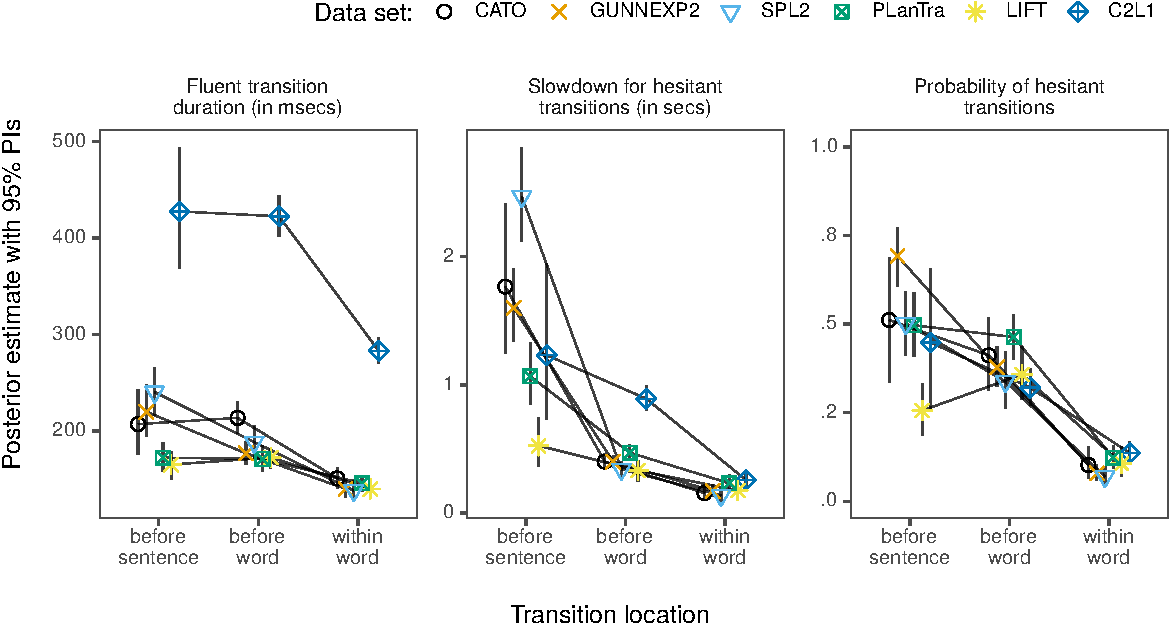
\includegraphics{manuscript_files/figure-latex/crossstudypost-1} 

}

\caption{Mixture model parameter estimates across studies. Distributions of parameter estimates are represented as posterior mean and 95\% probability interval (PI). Estimates for the CATO dataset were calculated for the non-dyslexic group, unmasked condition; also the GUNNEXP2 estimtes represent the unmasked condition; SPL2 estimates are for the L1 group. Axes for transitions durations are log-scaled for visability.}\label{fig:crossstudypost}
\end{figure}

In the following we evaluate differences between transition locations
for all three mixture model parameters. Figure \ref{fig:crossstudypost}
shows largely the same patterns (with caveats) for keystroke interval
estimates by transition location across data sets for all three mixture
model parameters. We found that hesitations appear more frequently at
before-word transitions than within words across data sets (all BFs
\textgreater{} 100). Also hesitations are longer at before-sentence
transitions compared to before-word transitions (all BFs \textgreater{}
100; except for C2L1: BF = 0.35 and LIFT = 2.14) and before-word
transitions compared to within-word transitions (all BF \textgreater{}
10; except for LIFT: BF = 0.71). Further, we observed that fluent
key-transitions are slower at before-word and before-sentence locations
compared to within-word locations (all BFs \textgreater{} 100) but there
is generally no evidence for a difference for fluent transitions for
before-sentence transitions compared to before-word transitions (BFs
\textless{} 0.08; except for SPL2: BF \textgreater{} 100 and GUNNEXP2:
BF \textgreater{} 100). The full results of these pairwise comparisons
can be found in Table \ref{tab:loceffect}.

Hesitation duration tends to be longer at before-sentence locations
compared to before-word locations (except for data sets C2L1 and LIFT)
and longer for before-word locations compared to within-word locations
(except for the LIFT data set). However, for most data set there is
negligible evidence for the idea that writers pause more frequently at
before-sentence locations compared to before-word locations (except for
data sets SPL2 and GUNNEXP2). This is interesting because it is
generally believed that pausing behaviour is associated with syntactic
edges such that more and longer pauses are predicted for key transitions
at larger syntactic edges following the pattern before-sentence \(>\)
before-word \(>\) within-word. In fact, the data set LIFT showed less
pausing before sentences compared to before words. In brief, while
keystroke transitions and pauses tend to be longer and more frequent at
before-word locations compared to within-word transitions, it is not
clear in which contexts keystroke transitions are before-sentence
locations are slower, and their hesitations are longer and more
frequent.

Outstanding is the overall substantially longer fluent transitions for
the C2L1 data. This is presumably reflecting that the population that
this sample is from was the youngest among our data sets presumably
involving the least experienced writers in our data pool. Hesitation
duration and frequencies were similar to the other data sets. There are
some inconsistencies for fluent before-sentence transitions compared to
before-word transitions. Some data sets show before-sentence slowdowns
for fluent transition compared to words. These inconsistencies could, to
some extent, be explained on the basis that data sets differ as to
whether before-sentence transitions involve complex key combination
involve the mean or sum of transitions between space, shift and / or the
sentence-initial letters. In particular, some data include the character
key following the shift key at before sentence location (PLanTra, LIFT)
but others did not scope over the character following the shift key
(CATO, C2L1, SPL2, GUNNEXP2). Notice though that for the data sets
PLanTra and LIFT, there was no evidence for a consistent differences
between before-sentence and before-word transitions (except for longer
hesitations in the PLanTra dataset).

To address this finding, and inconsistency in how before-sentence
transitions were timed, we test to what extent this difference affected
the modelling results for the SPL2 data set. The results are shown in
Appendix \ref{key-combination-effect-unconstrained-mixture-model}. We
found that including the character following the shift key substantially
extends both the transition duration and the hesitation duration but not
the hesitation frequency. However, this conflicts with the absence of
differences in data sets that included the character following shift at
before-sentence transitions (PLanTra, LIFT). In other words, it is
unlikely that patterns in our results can be explained on the basis of
how before-keystroke transitions were operationalised (complex
key-combinations at before-sentence locations).

\blandscape

\begin{center}
\begin{ThreePartTable}

\begin{TableNotes}[para]
\normalsize{\textit{Note.} PI = probability intervals. BF = evidence in favour of the alternative hypothesis over the null hypothesis.}
\end{TableNotes}

\footnotesize{

\begin{longtable}{lrrrrrr}\noalign{\getlongtablewidth\global\LTcapwidth=\longtablewidth}
\caption{\label{tab:loceffect}Effect of transition location on keystroke intervals. Differences are shown on log scale (for transition durations) and logit scale for probability of hesitant transitions. 95\% PIs in brackets.}\\
\toprule
 \multicolumn{1}{c}{ } & \multicolumn{2}{c}{Fluent transitions} & \multicolumn{2}{c}{Hesitation slowdown} & \multicolumn{2}{c}{Hesitation probability} \\
\cmidrule(r){1-1} \cmidrule(r){2-3} \cmidrule(r){4-5} \cmidrule(r){6-7}
Comparison & Est. [95\% PIs] & BF & Est. [95\% PIs] & BF & Est. [95\% PIs] & BF\\
\midrule
\endfirsthead
\caption*{\normalfont{Table \ref{tab:loceffect} continued}}\\
\toprule
 \multicolumn{1}{c}{ } & \multicolumn{2}{c}{Fluent transitions} & \multicolumn{2}{c}{Hesitation slowdown} & \multicolumn{2}{c}{Hesitation probability} \\
\cmidrule(r){1-1} \cmidrule(r){2-3} \cmidrule(r){4-5} \cmidrule(r){6-7}
Comparison & Est. [95\% PIs] & BF & Est. [95\% PIs] & BF & Est. [95\% PIs] & BF\\
\midrule
\endhead
\textbf{C2L1} &  &  &  &  &  & \\
\ \ \ before sentence vs word & 0.01 [-0.13, 0.15] & 0.07 & 0.21 [-0.13, 0.54] & 0.35 & 0.54 [-0.31, 1.43] & 0.89\\
\ \ \ before vs within word & 0.4 [0.38, 0.42] & > 100 & 0.49 [0.39, 0.58] & > 100 & 1.1 [0.76, 1.44] & > 100\\
\textbf{CATO (non-dyslexic, unmasked)} &  &  &  &  &  & \\
\ \ \ before sentence vs word & -0.03 [-0.18, 0.11] & 0.08 & 1.19 [0.88, 1.49] & > 100 & 0.41 [-0.44, 1.27] & 0.67\\
\ \ \ before vs within word & 0.35 [0.31, 0.38] & > 100 & 0.35 [0.14, 0.54] & 17.48 & 1.83 [1.19, 2.49] & > 100\\
\textbf{GUNNEXP2 (unmasked)} &  &  &  &  &  & \\
\ \ \ before sentence vs word & 0.22 [0.12, 0.32] & > 100 & 0.93 [0.78, 1.07] & > 100 & 1.32 [0.86, 1.78] & > 100\\
\ \ \ before vs within word & 0.23 [0.21, 0.25] & > 100 & 0.38 [0.21, 0.54] & > 100 & 1.97 [1.59, 2.37] & > 100\\
\textbf{LIFT} &  &  &  &  &  & \\
\ \ \ before sentence vs word & -0.04 [-0.13, 0.05] & 0.07 & 0.35 [0.05, 0.72] & 2.14 & -0.49 [-1.03, 0] & 1.63\\
\ \ \ before vs within word & 0.21 [0.13, 0.27] & > 100 & 0.26 [-0.16, 0.55] & 0.71 & 1.56 [1.02, 2.16] & > 100\\
\textbf{PLanTra} &  &  &  &  &  & \\
\ \ \ before sentence vs word & 0.01 [-0.09, 0.11] & 0.07 & 0.65 [0.46, 0.83] & > 100 & 0.13 [-0.25, 0.53] & 0.25\\
\ \ \ before vs within word & 0.16 [0.1, 0.21] & > 100 & 0.37 [0.2, 0.54] & > 100 & 1.83 [1.48, 2.17] & > 100\\
\textbf{SPL2 (L1)} &  &  &  &  &  & \\
\ \ \ before sentence vs word & 0.24 [0.17, 0.31] & > 100 & 1.39 [1.25, 1.52] & > 100 & 0.69 [0.17, 1.19] & 8.01\\
\ \ \ before vs within word & 0.31 [0.28, 0.34] & > 100 & 0.35 [0.14, 0.54] & 16.25 & 1.94 [1.4, 2.5] & > 100\\
\bottomrule
\addlinespace
\insertTableNotes
\end{longtable}

}

\end{ThreePartTable}
\end{center}
\elandscape
\end{appendix}

\clearpage
\makeatletter
\efloat@restorefloats
\makeatother


\begin{appendix}
\section{}
\hypertarget{key-combination-effect-unconstrained-mixture-model}{%
\subsection{Key-combination effect (unconstrained mixture
model)}\label{key-combination-effect-unconstrained-mixture-model}}

The analysed datasets differ to the extent that keystroke intervals at
before sentence location sometimes did (PLanTra, LIFT) or did not (CATO,
C2L1, SPL2, GUNNEXP2) scope over the character following the shift key.
In other words, the pause before sentences sumed across two key
intervals in the PLanTra and LIFT data, namely
\texttt{\_\^{}{[}shift{]}\^{}C} but only involved one key interval,
namely \texttt{\_\^{}{[}shift{]}} for the remaining datasets. Therefore,
longer or more frequent pauses at before-sentence locations compared to
before-word locations can be explained without reference to linguistic
edges. Also there is a possibility that some inconsistencies in our
findings can be explained on the basis of including the keystroke
following shift.

Therefore we compared whether the different patterns can be explain on
the basis of the additional keystroke involved in before-sentence
transitions. We compared the SPL2 data including and excluding the
keystroke after shift. Although we modelled all transition locations, we
present only before-sentence transitions below as there was, as one
would expect, no difference at word locations. The results of this
comparison can be found in Table \ref{tab:shiftcellmeans2}.

\begin{center}
\begin{ThreePartTable}

\begin{TableNotes}[para]
\normalsize{\textit{Note.} PIs are probability intervals. BF is the evidence in favour of the alternative hypothesis over the null hypothesis.}
\end{TableNotes}

\footnotesize{

\begin{longtable}{lrrr}\noalign{\getlongtablewidth\global\LTcapwidth=\longtablewidth}
\caption{\label{tab:shiftcellmeans2}Mixture model estimates for key transitions. Cell means are shown for transitions that do and do not involve the transition to the character following shift in msecs for fluent key-transitions, the slowdown for long transitions and the probability of hesitant transitions. The difference for including the transition duration to the character after shift is shown on log scale (for transition durations) and logit scale for probability of hesitant transitions. 95\% PIs in brackets.}\\
\toprule
Language & \multicolumn{1}{c}{\_\textasciicircum{}[shift]} & \multicolumn{1}{c}{Difference} & \multicolumn{1}{c}{BF}\\
\midrule
\endfirsthead
\caption*{\normalfont{Table \ref{tab:shiftcellmeans2} continued}}\\
\toprule
Language & \multicolumn{1}{c}{\_\textasciicircum{}[shift]} & \multicolumn{1}{c}{Difference} & \multicolumn{1}{c}{BF}\\
\midrule
\endhead
Fluent transitions &  &  & \\
\ \ \ L1 & 159 [147, 172] & 0.48 [0.34, 0.63] & > 100\\
\ \ \ L2 & 159 [147, 172] & 0.41 [0.19, 0.63] & 46.08\\
Hesitation duration &  &  & \\
\ \ \ L1 & 1,281 [1,082, 1,496] & -0.46 [-0.61, -0.3] & > 100\\
\ \ \ L2 & 1,802 [1,557, 2,073] & -0.34 [-0.51, -0.17] & > 100\\
Hesitation probability &  &  & \\
\ \ \ L1 & .78 [.69, .86] & 0.49 [-0.04, 1.03] & 1.43\\
\ \ \ L2 & .92 [.87, .96] & 0.48 [-0.16, 1.13] & 0.94\\
\bottomrule
\addlinespace
\insertTableNotes
\end{longtable}

}

\end{ThreePartTable}
\end{center}

Overall, fluent transition duration and the hesitation duration were
affected by whether or not the sentence-initial transition include the
character following shift. Fluent key transitions were substantially
longer when including the interval following the shift key. The slowdown
for hesitations was affected too but the difference is numerically
small. There was no conclusive evidence for an increased hesitation
probability.
\end{appendix}

\clearpage
\makeatletter
\efloat@restorefloats
\makeatother


\begin{appendix}
\section{}
\hypertarget{simulation}{%
\subsection{Simulation}\label{simulation}}

A possible concern with these results -- substantially better predictive
performance for two-distribution mixture models -- is that, in
principle, as the mixture model has more parameters it might always lead
to a better fit. We addressed this concern before by using
cross-validation techniques for model comparison which is preventing
overfitting models. To address this concern we repeated a comparison for
a single distribution model and a two-distrobutionsl mixture model for
two sets of simulated data that were simulated either with a single
distribution or two-distributional process at heart. In other words,
this allows us to test the predictive performance of our models in a
context where we know the true underlying data generating process --
single distribution vs two distributions -- and we can test whether
these models can successfully uncover the true parameter value.

In particular, the first data set was simulated using a
two-distributions mixture model with two mixture components similar to
the process described above (equations in \ref{eq:bimodcon} and
\ref{eq:bimoduncon}). This process and the corresponding Bayesian model
is summarised in equation \ref{eq:simmog}.

\begin{equation}
\begin{aligned}
\label{eq:simmog}
\text{y} \sim\text{ } & \theta \cdot \text{logN}(\beta + \delta, \sigma^2_1) +\\
& (1 - \theta) \cdot \text{logN}(\beta, \sigma^2_2)\\
\text{constraint: } & \delta, \sigma_\text{2}^2, \sigma_\text{1}^2>0\\
        & \sigma_{1}^2 > \sigma_{2}^2
\end{aligned}
\end{equation}

This model is largely identical to the models before but reduced to its
main parameters (but not mixed effects for participants). The model
includes two log-normal distributions with a mixing proportion
\(\theta\) of which the distribution of shorter values has a mean of
\(\beta\) and a standard deviation \(\sigma^2_2\); the second
distribution of longer values is constrained to have a mean that is
larger by a factor of \(\delta\) and has a larger standard deviation
\(\sigma^2_1\).

The second data set was generated with a single distribution
log-Gaussian process. The model and its corresponding Bayesian model is
summarised in equation \ref{eq:simuv}.

\begin{equation}
\begin{aligned}
\label{eq:simuv}
\text{y} \sim\text{ }& \text{logN}(\beta, \sigma^2)\\
\text{constraint: } & \sigma^2>0
\end{aligned}
\end{equation}

Again, this model is a simplified version of the single distribution
models used in the main analysis. The model assumes a log-Gaussian
distribution with a mean parameter \(\beta\) and a standard deviation
\(\sigma^2\).

The parameter values used for each of the two data simulations can be
found in Table \ref{tab:simparam}. The simulated data are visualised in
Figure \ref{fig:simdata}. Parameter values were chosen so that the
simulated data are roughly similarly distributed to keystroke
transitions.

\begin{figure}

{\centering 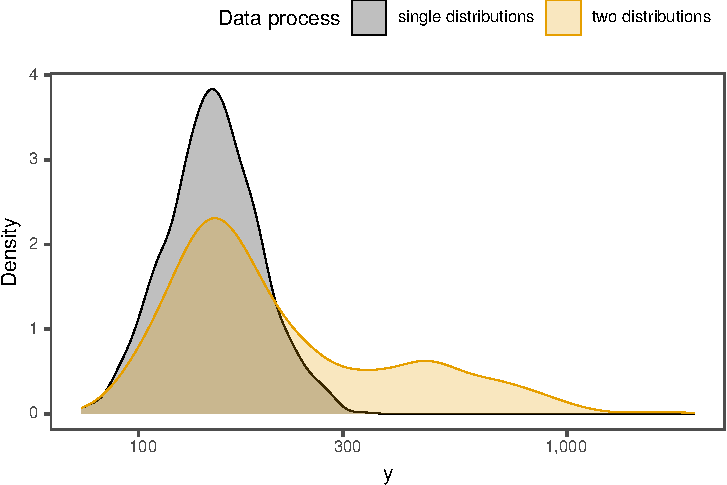
\includegraphics{manuscript_files/figure-latex/simdata-1} 

}

\caption{Data simulated with a two-distribution (grey) and a single-distribution (yellow) random data generating process. The x-axis showing the outcome y was log-scaled for visability.}\label{fig:simdata}
\end{figure}

For each of these two data sets we simulated 1,000 observations. We run
2 models -- a two-distribution mixture model and a single-distribution
model -- each for both data sets. Models were run with 3 chains, with
each 6,000 iterations of which 3,000 were warmup. Estimates with 95\%
probability intervals are shown in Table \ref{tab:simparam}. The
parameters are shown by type of data generating process along with the
true parameter values. Parameter value estimates are shown by type of
Bayesian model. The results show that either of the two Bayesian models
succesfully uncovered the model parameters of the data with its
corresponding data generating process, as shown in Table
\ref{tab:simparam}, but less so when the model was applied to data
generated with the incorrect underlying process. Particularly the mixing
proportion \(\theta\) and the slowdown parameter \(\delta\) were not
uncovered at all by they single-distribution model.

\begin{table}[tbp]

\begin{center}
\begin{threeparttable}

\caption{\label{tab:simparam}Uncovered parameter estimates with 95\% probability interval (PI) and true parameter values for each simulated data set and by model and their respective parameters.}

\begin{tabular}{lrr}
\toprule
 & \multicolumn{2}{c}{Estimate with 95\% PI} \\
\cmidrule(r){2-3}
Parameter with true value & \multicolumn{1}{c}{Two-distributions model} & \multicolumn{1}{c}{Single-distributions model}\\
\midrule
Two-distributions data &  & \\
\ \ \ $\beta = 5$ & 5.02 [4.99, 5.04] & 4.93 [4.76, 5.01]\\
\ \ \ $\delta = 1$ & 1.04 [0.92, 1.14] & 0.13 [0.01, 0.3]\\
\ \ \ $\theta = .35$ & .33 [.28, .39] & .54 [.11, .92]\\
\ \ \ $\sigma^2_1 = 0.25$ & 0.25 [0.23, 0.27] & 0.22 [0.16, 0.25]\\
\ \ \ $\sigma^2_2 = 0.5$ & 0.49 [0.42, 0.57] & 0.25 [0.22, 0.3]\\
Single-distribution data &  & \\
\ \ \ $\beta = 5$ & 5.35 [5.32, 5.39] & 5 [4.99, 5.02]\\
\ \ \ $\sigma = 0.25$ & 0.6 [0.57, 0.63] & 0.25 [0.24, 0.26]\\
\bottomrule
\end{tabular}

\end{threeparttable}
\end{center}

\end{table}

We used LOO-CV to compare the predictive performance of the two models
for each data generating process. The model comparisons can be found for
each data generating process in Table \ref{tab:loossim}. The results
rule out the possibility that the mixture model does always lead to
higher predictive performance. Indeed, the mixture model showed a
slightly lower predictive performance for the data that were generated
with a single-distribution process. However, for the data generated with
a two-distribution mixture process, the mixture model shows a
substantially higher predictive performance. In fact, the ratio of
\(\Delta\widehat{elpd}\) and its standard error -- a \emph{z}-score
approximation -- reveals a value of 11.6 which is strong evidence in in
favour of the mixture model compared to the single-distribution model
(Sivula et al., 2020). In comparison, for the single-distribution data,
the single-distribution model was negligibly better than the
two-distribution mixture model which was evidence by a value of 0.77 for
the ratio of \(\Delta\widehat{elpd}\) and its standard error. Thus, as
the difference \(\Delta\widehat{elpd}\) between the model is negligible,
the single distribution is preferred by the law of parsimony.

\begin{table}[tbp]

\begin{center}
\begin{threeparttable}

\caption{\label{tab:loossim}Model comparisons by data set. The top row shows the models with the highest predictive performance for each data generating process. Standard error is shown in parentheses.}

\begin{tabular}{lrr}
\toprule
Model & \multicolumn{1}{c}{$\Delta\widehat{elpd}$} & \multicolumn{1}{c}{$\widehat{elpd}$}\\
\midrule
Data: Two-distribution mixture process &  & \\
\ \ \ Two-distribution mixture model & -- & -6,068 (41)\\
\ \ \ Single-distribution model & -191.3 (16.5) & -6,259 (38)\\
Data: Single-distribution process &  & \\
\ \ \ Single-distribution model & -- & -5,030 (24)\\
\ \ \ Two-distribution mixture model & -0.5 (0.7) & -5,030 (24)\\
\bottomrule
\addlinespace
\end{tabular}

\begin{tablenotes}[para]
\normalsize{\textit{Note.} $\widehat{elpd}$ = predictive performance indicated as expected log pointwise predictive density; $\Delta\widehat{elpd}$ = difference in predictive performance relative to the model with the highest predictive performance in the top row.}
\end{tablenotes}

\end{threeparttable}
\end{center}

\end{table}
\end{appendix}

\end{document}
